\documentclass[9pt,portrait]{article}
\usepackage{beamerarticle} % makes slides into article

%% xcolor Option Clash issue
%	Do not include xcolor,, tikz-qtree, todonotes, here do it after beamerarticle
\usepackage{multicol}
\usepackage{booktabs}
\usepackage{calc}
\usepackage{ifthen}
\usepackage[portrait]{geometry}
\usepackage{hyperref}
\usepackage{color}
\usepackage{enumitem}
\usepackage{textcomp} 				% copyleft symbol
\usepackage{verbatim}
\usepackage{adjustbox} 				% for resizebox to adjust table figure content
\usepackage{enumitem}				% margin free lists
\usepackage{amsmath}
\usepackage{mathrsfs}
\usepackage{csvsimple}				% importing csv as table
\usepackage{textcomp} 				% copyleft symbol
\usepackage{graphicx}
\usepackage{etoolbox} % conditional inclusions

\usepackage{media9}
 \usepackage{multimedia}
 \usepackage{makecell}
 \usepackage{listings}
%  \usepackage{color}
 
\definecolor{codegreen}{rgb}{0,0.6,0}
\definecolor{codegray}{rgb}{0.5,0.5,0.5}
\definecolor{codepurple}{rgb}{0.58,0,0.82}
\definecolor{backcolour}{rgb}{.914, .89, .957} % pale purple

\definecolor{mygreen}{rgb}{0,0.6,0}
\definecolor{mygray}{rgb}{0.5,0.5,0.5}
\definecolor{mymauve}{rgb}{0.58,0,0.82}

\lstdefinestyle{mystyle}{
  backgroundcolor=\color{backcolour},   % choose the background color; you must add \usepackage{color} or \usepackage{xcolor}; should come as last argument
  basicstyle=\footnotesize\ttfamily,       % the size of the fonts that are used for the code
  breakatwhitespace=true,          % sets if automatic breaks should only happen at whitespace
  breaklines=true,                 % sets automatic line breaking
  captionpos=b,                    % sets the caption-position to bottom
  commentstyle=\color{mygreen},    % comment style
  deletekeywords={...},            % if you want to delete keywords from the given language
  escapeinside={\%*}{*)},          % if you want to add LaTeX within your code
  extendedchars=true,              % lets you use non-ASCII characters; for 8-bits encodings only, does not work with UTF-8
  frame=single,	                   % adds a frame around the code
  keepspaces=true,                 % keeps spaces in text, useful for keeping indentation of code (possibly needs columns=flexible)
  keywordstyle=\color{blue},       % keyword style
  language=Python,                 % the language of the code
  morekeywords={*,...},            % if you want to add more keywords to the set
  % numbers=left,                    % where to put the line-numbers; possible values are (none, left, right)
  % numbersep=5pt,                   % how far the line-numbers are from the code
  % numberstyle=\tiny\color{mygray}, % the style that is used for the line-numbers
  rulecolor=\color{black},         % if not set, the frame-color may be changed on line-breaks within not-black text (e.g. comments (green here))
  showspaces=false,                % show spaces everywhere adding particular underscores; it overrides 'showstringspaces'
  showstringspaces=false,          % underline spaces within strings only
  showtabs=false,                  % show tabs within strings adding particular underscores
  stepnumber=2,                    % the step between two line-numbers. If it's 1, each line will be numbered
  stringstyle=\color{codepurple},  % string literal style
  tabsize=2,	                   % sets default tabsize to 2 spaces
  columns=fullflexible,
  linewidth=0.98\linewidth,        % Box width
  aboveskip=10pt,	   			   % Space before listing 
  belowskip=-15pt,	   			   % Space after listing  
  xleftmargin=.02\linewidth,  
  title=\lstname                   % show the filename of files included with \lstinputlisting; also try caption instead of title
}


% \definecolor{codegreen}{rgb}{0,0.6,0}
% \definecolor{codegray}{rgb}{0.5,0.5,0.5}
% \definecolor{codepurple}{rgb}{0.58,0,0.82}
% %\definecolor{backcolour}{rgb}{0.95,0.95,0.92} % faint postman color
% \definecolor{backcolour}{rgb}{.914, .89, .957} % pale purple
% %\lstset{basicstyle=\footnotesize\ttfamily}

% \lstdefinestyle{mystyle}{
    % backgroundcolor=\color{backcolour},   
    % commentstyle=\color{codegreen},
    % keywordstyle=\color{magenta},
    % numberstyle=\tiny\color{codegray},
    % stringstyle=\color{codepurple},
    % basicstyle= \tiny\ttfamily %\scriptsize\ttfamily, %\footnotesize,  % the size of the fonts that are used for the code
    % breakatwhitespace=true,  % sets if automatic breaks should only happen at whitespace        
    % breaklines=true, % sets automatic line breaking   
    % linewidth=\linewidth,	
    % captionpos=b,                    
    % keepspaces=true,% keeps spaces in text, useful for keeping indentation                
% %    numbers=left,                  
    % numbers=none,  
% %    numbersep=5pt,                  
    % showspaces=false,                
    % showstringspaces=false,
    % showtabs=false,                  
    % tabsize=2
% }
\lstset{style=mystyle}


%\lstset{basicstyle=\footnotesize\ttfamily}

\newtoggle{VideoFrames}
\togglefalse{VideoFrames}


\newtoggle{CopyrightPictures}
\togglefalse{CopyrightPictures}

\hypersetup{ % remove ugly hyperlink boxes
    colorlinks,
    linkcolor={red!50!black},
    citecolor={blue!50!black}%,
    %urlcolor={green!80!black}
}

% This sets page margins to .5 inch if using letter paper, and to 1cm
% if using A4 paper. (This probably isn't strictly necessary.)
% If using another size paper, use default 1cm margins.
\ifthenelse{\lengthtest { \paperwidth = 8.5in}}
	{ \geometry{top=.2in,left=.25in,right=.25in,bottom=.5in} }
	{\ifthenelse{ \lengthtest{ \paperwidth = 290mm}}
		{\geometry{top=1cm,left=1cm,right=1cm,bottom=2cm} }
		{\geometry{top=1cm,left=1cm,right=1cm,bottom=2cm} }
	}

% % Turn off header and footer
% \pagestyle{empty}

\usepackage{fancyhdr}   % Package to customize headers and footers
% Turn ON header and footer
\pagestyle{fancy}

% Add a line above the footer
\renewcommand{\footrulewidth}{0.4pt}  % Set the line thickness (adjust as needed)
% Set footer content
\fancyfoot[C]{\textit{Yogesh Haribhau Kulkarni}} % Centered footer text
\fancyfoot[R]{\thepage}                       % Page number on the right
\fancyfoot[L]{\textit{\href{http://www.yogeshkulkarni.com}{yogeshkulkarni@yahoo.com}}} % Centered footer text

% Optional: Set header if needed
%\fancyhead[L]{\textit{Your Header Text Here}} % Header text on the left
 

% Redefine section commands to use less space
\makeatletter
\renewcommand{\section}{\@startsection{section}{1}{0mm}%
                                {-1ex plus -.5ex minus -.2ex}%
                                {0.5ex plus .2ex}%x
                                {\normalfont\large\bfseries}}
\renewcommand{\subsection}{\@startsection{subsection}{2}{0mm}%
                                {-1explus -.5ex minus -.2ex}%
                                {0.5ex plus .2ex}%
                                {\normalfont\normalsize\bfseries}}
\renewcommand{\subsubsection}{\@startsection{subsubsection}{3}{0mm}%
                                {-1ex plus -.5ex minus -.2ex}%
                                {1ex plus .2ex}%
                                {\normalfont\small\bfseries}}
\makeatother

% Define BibTeX command
\def\BibTeX{{\rm B\kern-.05em{\sc i\kern-.025em b}\kern-.08em
    T\kern-.1667em\lower.7ex\hbox{E}\kern-.125emX}}

% Don't print section numbers
\setcounter{secnumdepth}{0}

\newcommand{\code}[1]{\par\vskip0pt plus 1filll \footnotesize Code:~\itshape#1}


\setlength{\parindent}{0pt}
\setlength{\parskip}{0pt plus 0.5ex}
\setlength\columnsep{30pt}

\usepackage{tcolorbox}  % For creating fancy boxes
\usepackage{tikz}       % For drawing borders

% Define a fancy style for cover pages
\tcbuselibrary{skins, breakable, theorems}
\tcbset{
    coverstyle/.style={
        enhanced,
        colframe=black,
        colback=white,
        coltitle=black,
        fonttitle=\bfseries\LARGE,
        fontupper=\normalsize,
        boxrule=1mm,
        width=\textwidth,
        arc=4mm,
        boxsep=5mm,
        outer arc=0mm,
        attach boxed title to top center={yshift=-0.5cm},
        boxed title style={colframe=black, colback=white, boxrule=0mm},
    }
}
\usepackage{polyglossia}
\setdefaultlanguage{sanskrit}
\setotherlanguage{english}

\usepackage{fontspec}
\setmainfont{Segoe UI}

% Devanagari Fonts
\newfontfamily\devanagarifont[Script=Devanagari]{Nakula}
\newfontfamily\devanagarifontsf[Script=Devanagari]{Nakula}
\newfontfamily\devanagarifonttt[Script=Devanagari]{Nakula}
\newfontfamily\devtransl[Mapping=DevRom]{Segoe UI}


% Sharada Fonts
\newfontfamily\sharadafont[Script=Sharada]{Noto Sans Sharada}

\graphicspath{{images/}}


\begin{document}
\footnotesize


\begin{center}
\Large{\textbf{Shrimath Yoga - Krishna Prakash}} 
\end{center}

\begin{multicols}{2}
% %%%%%%%%%%%%%%%%%%%%%%%%%%%%%%%%%%%%%%%%%%%%%%%%%%%%%%%%%%%%%%%%%%%%%%%%%%%%%%%%%%
% \begin{frame}[fragile]\frametitle{}
% \begin{center}
% {\Large Notes from Teachings of Krishna Prakash of Shrimath}
% \end{center}
% \end{frame}

% %%%%%%%%%%%%%%%%%%%%%%%%%%%%%%%%%%%%%%%%%%%%%%%%%%%%%%%%%%%
% \begin{frame}[fragile]\frametitle{Starting Yoga}

	% \begin{itemize}
	% \item Yoga Sadhna is An Endless Ocean	
	% \item You cannot be a Yoga Teacher/Guru just after training or certification, practice it for years (12), experience the benefits, then only teach.
	% \item Small Sized Yoga Classes is a Must
	% \item Meditation instructions lack emphasis on posture.
	% \item Still Your Body and Steady Mind
	% \item Persist with spiritual practices Long Enough
	% \item Guru emphasizes endless hours, and dedication for yoga.
	% \item Without steadiness, meditation cannot happen e.g. curd sets when still
	% \item Asana brings steadiness and Pranayama brings lightness, pratyahara brings witness-bhava
	% \item Pavanmuktasana series by Satyananda, of 34 Asanas To Start Yoga Journey
	% \end{itemize}

% {\tiny (Ref:  I Did yoga for 7 Days Following A Yogi's Advice- With ‪@ShrimathYoga‬  spirituality - Tathastu - Secrets of Bharat)}

% \end{frame}

% %%%%%%%%%%%%%%%%%%%%%%%%%%%%%%%%%%%%%%%%%%%%%%%%%%%%%%%%%%%
% \begin{frame}[fragile]\frametitle{Immunity}

% \begin{columns}
    % \begin{column}[T]{0.6\linewidth}
		% \begin{itemize}
		% \item 340 important pressure points on the body with which health can be managed. 28 are on palms. Clapping for upto 20 minutes before meals
		% \item 'PraN Mudra' (thumb and last two small fingers touching) 12 minutes
		% \item 'Ling Mudra' (fist clasped, left thumb upward, keep at naval) 12 minutes
		% \item Bhramari Pranayam + Khechari Mudra, inhale without sound, exhale with bee sound from tight throat. 7 minutes, 3 times a day.
		% \end{itemize}

    % \end{column}
    % \begin{column}[T]{0.4\linewidth}
		% \begin{center}
		% 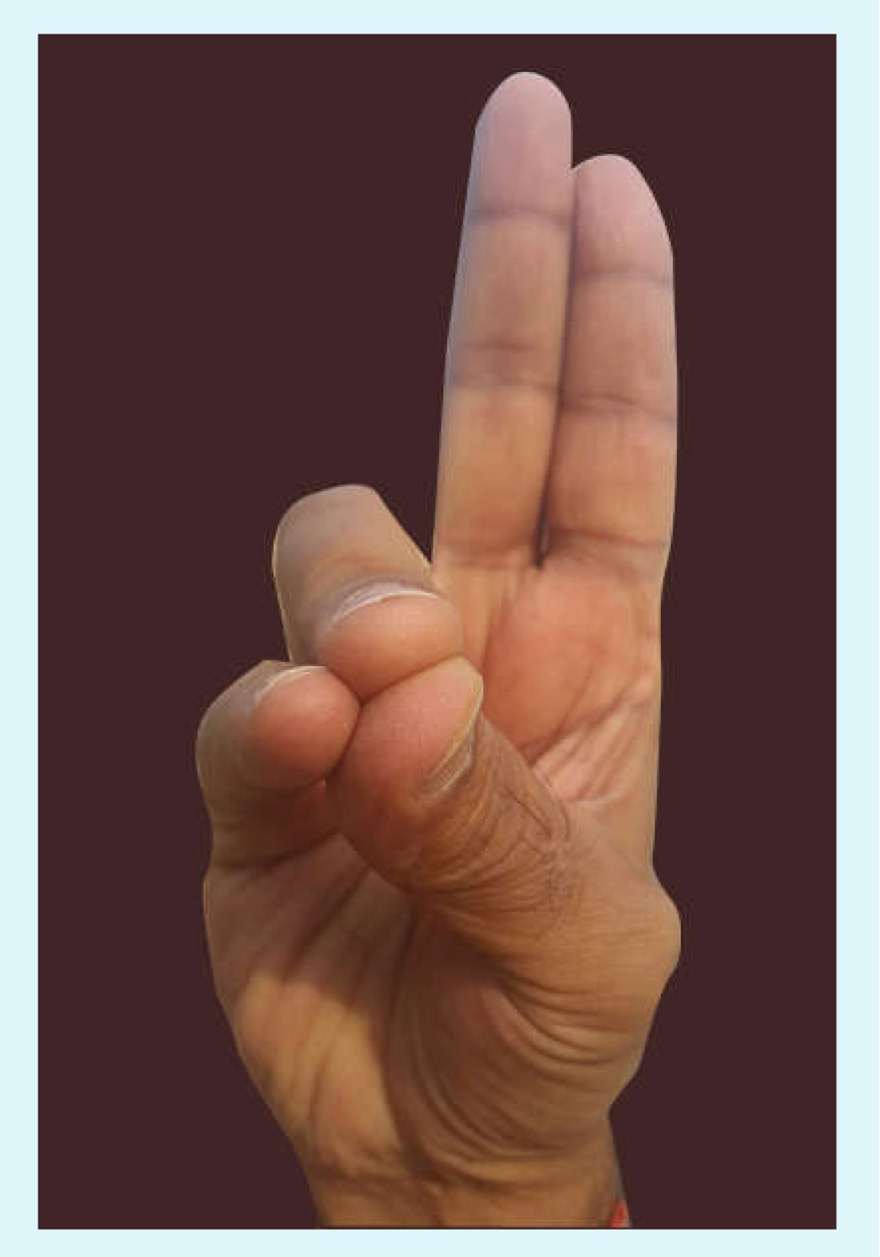
\includegraphics[width=0.4\linewidth,keepaspectratio]{pranmudra}
		
		% 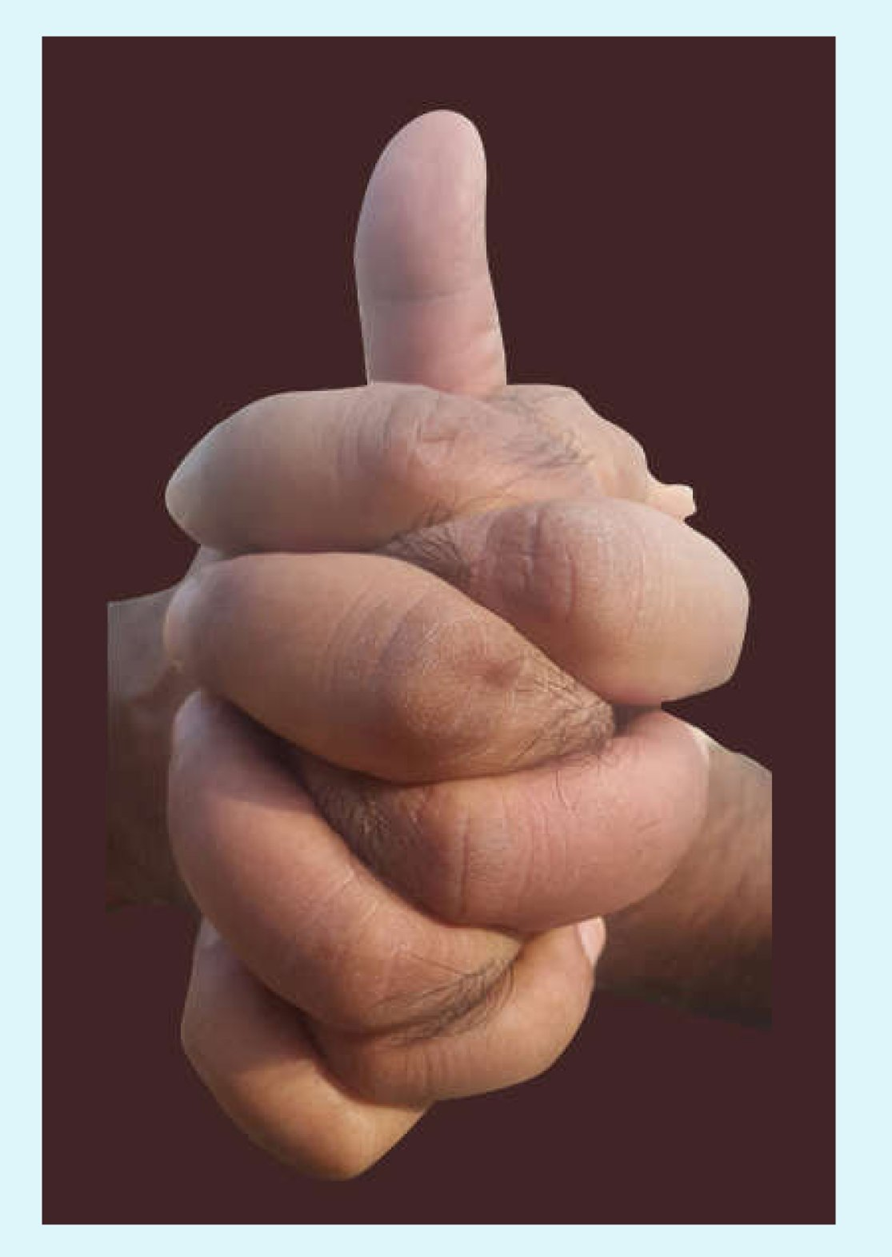
\includegraphics[width=0.4\linewidth,keepaspectratio]{lingmudra}
		
		% \end{center}	
    % \end{column}
  % \end{columns}
  


% {\tiny (Ref:  Building Immunity 2.0 - Shrimath Yoga)}

% \end{frame}

%%%%%%%%%%%%%%%%%%%%%%%%%%%%%%%%%%%%%%%%%%%%%%%%%%%%%%%%%%%%%%%%%%%%%%%%%%%%%%%%%%
\begin{frame}[fragile]\frametitle{}
\begin{center}
{\Large Inner Silence}
\end{center}

{\tiny (Ref:  Master Class on Antar Mouna Level 1 - Shrimath Yoga)}

\end{frame}

%%%%%%%%%%%%%%%%%%%%%%%%%%%%%%%%%%%%%%%%%%%%%%%%%%%%%%%%%%%
\begin{frame}[fragile]\frametitle{What is Inner Silence?}
    \begin{itemize}
        \item Practice of Pratyahara प्रत्याहार : Withdrawing is difficult as our nature is to seek knowledge.
        \item Vedanta: Our Ultimate Reality is Sat Chid Anand. सत् चित् आनन्द 
        \item \textbf{Sat सत्} - Pure existence, why we wish to live forever.
        \item \textbf{Chit चित् } - Consciousness, reason for our thirst for knowledge.
        \item \textbf{Ananda} - Pure bliss, reason we avoid sadness.
    \end{itemize}
\end{frame}

%%%%%%%%%%%%%%%%%%%%%%%%%%%%%%%%%%%%%%%%%%%%%%%%%%%%%%%%%%%
\begin{frame}[fragile]\frametitle{Understanding Sat सत्  Chit चित्  Anand आनन्द}
    \begin{itemize}
        \item We fear death because of our attachment to existence (Sat सत्).
        \item Knowledge is innate; absence of it makes us restless (Chit चित् ).
        \item We resist sadness as our nature is bliss (Ananda आनन्द).
        \item Stress, annoyance, and irritation arise from deviation from bliss.
    \end{itemize}
\end{frame}

%%%%%%%%%%%%%%%%%%%%%%%%%%%%%%%%%%%%%%%%%%%%%%%%%%%%%%%%%%%
\begin{frame}[fragile]\frametitle{Ocean Analogy \& Realization}
    \begin{itemize}
        \item Waves exist only near the shore; deep ocean remains still.
        \item Inner silence grows with experience and realization.
        \item Excess money, fame, or power do not equate to true calmness.
        \item True peace comes from within, not from external achievements.
    \end{itemize}
\end{frame}

%%%%%%%%%%%%%%%%%%%%%%%%%%%%%%%%%%%%%%%%%%%%%%%%%%%%%%%%%%%
\begin{frame}[fragile]\frametitle{Withdrawal - The Key to Inner Silence}
    \begin{itemize}
        \item Managing the five senses is the first level of inner silence.
        \item Sensory pulls appear enticing but cause distractions.
        \item Regular withdrawal helps recuperate and maintain balance.
        \item Use senses to transcend distractions, not be controlled by them.
    \end{itemize}
\end{frame}

%%%%%%%%%%%%%%%%%%%%%%%%%%%%%%%%%%%%%%%%%%%%%%%%%%%%%%%%%%%
\begin{frame}[fragile]\frametitle{Antar Mouna अंतर मौन  - The Battle Within}
    \begin{itemize}
        \item Practiced amidst daily life, not in isolation.
        \item 6 levels of Antar Mouna:
        \item \textbf{Level 1}: Live with sensory pulls, accept distractions.
        \item Do not give control of your mind to external factors.
        \item Listing and observing distractions helps detach from them.
        \item Avoidance increases suffering; face challenges and evolve.
    \end{itemize}
\end{frame}

%%%%%%%%%%%%%%%%%%%%%%%%%%%%%%%%%%%%%%%%%%%%%%%%%%%%%%%%%%%
\begin{frame}[fragile]\frametitle{Developing Inner Silence}
    \begin{itemize}
        \item Swami Satyananda स्वामी सत्यानंद : Inner silence $=$ mind aware of external sounds.
        \item Awareness of sounds brings moments of quietness within.
        \item Gradually, duration of inner silence increases.
        \item Some external sounds will always exist; accept and transcend them.
    \end{itemize}
\end{frame}

%%%%%%%%%%%%%%%%%%%%%%%%%%%%%%%%%%%%%%%%%%%%%%%%%%%%%%%%%%%
\begin{frame}[fragile]\frametitle{Prayer \& Practice}
    \begin{itemize}
        \item Ask God for energy to remain present in the moment.
        \item Prayer $+$ practice cultivates humility.
        \item Antar Mouna अंतर मौन Level 1: Eyes closed, smile, listen to sounds.
        \item Distractions will arise; bring awareness back gently.
        \item Witness, don’t resist; cultivate patience and kindness.
    \end{itemize}
\end{frame}

%%%%%%%%%%%%%%%%%%%%%%%%%%%%%%%%%%%%%%%%%%%%%%%%%%%%%%%%%%%
\begin{frame}[fragile]\frametitle{Decision-Making \& Sensory Control}
    \begin{itemize}
        \item Pause for 2-4 minutes before acting on sensory impulses.
        \item Awareness of senses refines speech, relationships, and choices.
        \item Right understanding of sound improves communication and knowledge.
        \item Better taste awareness naturally improves health and well-being.
    \end{itemize}
\end{frame}

%%%%%%%%%%%%%%%%%%%%%%%%%%%%%%%%%%%%%%%%%%%%%%%%%%%%%%%%%%%
\begin{frame}[fragile]\frametitle{Cultivating Emotional Balance}
    \begin{itemize}
        \item Self-awareness prevents emotional triggers from controlling us.
        \item We are our own saviors; no one else can do it for us.
        \item Antar Mouna अंतर मौन Level 1 builds emotional resilience through practice.
        \item Like agriculture, emotions need daily cultivation and care.
    \end{itemize}
\end{frame}

%%%%%%%%%%%%%%%%%%%%%%%%%%%%%%%%%%%%%%%%%%%%%%%%%%%%%%%%%%%
\begin{frame}[fragile]\frametitle{The Power of One}
    \begin{itemize}
        \item Depth matters more than breadth in spiritual practices.
        \item Focus on one mantra मंत्र , one pranayama प्राणायाम , one technique.
        \item Meditation is the result, not the goal; focus on the process.
        \item Rushing meditation hinders progress; patience is key.
    \end{itemize}
\end{frame}

%%%%%%%%%%%%%%%%%%%%%%%%%%%%%%%%%%%%%%%%%%%%%%%%%%%%%%%%%%%
\begin{frame}[fragile]\frametitle{Response vs Reaction}
    \begin{itemize}
        \item Antar Mouna creates moments of peace amidst chaos.
        \item In silence, personal realizations emerge.
        \item Situations won’t change, but our response can evolve.
        \item Transition from reacting emotionally to responding mindfully.
    \end{itemize}
\end{frame}


%%%%%%%%%%%%%%%%%%%%%%%%%%%%%%%%%%%%%%%%%%%%%%%%%%%%%%%%%%%
\begin{frame}[fragile]\frametitle{Summary}
		\begin{itemize}
		\item Part of Pratyahara (withdrawal of senses).
		\item Our attributes: We always seek to know, we wish to live forever and know what we don't know, even gossip is ok. We want to be happy.
		\item Level 1: learn to live with sensory pulls and pushes. Accept distractions. Going to retreat is running away from reality. We cannot change 'outside'. Be immune to it by being aware. Stand there in the problems. Be witness like a traffic police.
		\item Summary:
			\begin{itemize}
			\item Lesser thoughts
			\item Clarity in thought without confusion.
			\item Lack of prejudice and being open.
			\item Ability to stay calm even when triggered 
			\item Non judgmental and not jumping to conclusions even without listening and knowing about a subject.
			\end{itemize}
		\end{itemize}
\end{frame}


%%%%%%%%%%%%%%%%%%%%%%%%%%%%%%%%%%%%%%%%%%%%%%%%%%%%%%%%%%%%%%%%%%%%%%%%%%%%%%%%%%
\begin{frame}[fragile]\frametitle{}
\begin{center}
{\Large ``Tapping Grace through Yoga Nidra योगनिद्रा'' }
\end{center}

{\tiny (Ref:  Grace \& Yoga Nidra by Shrimath Yoga)}

\end{frame}

%%%%%%%%%%%%%%%%%%%%%%%%%%%%%%%%%%%%%%%%%%%%%%%%%%%%%%%%%%%
\begin{frame}[fragile]\frametitle{Part 1}

\begin{itemize}
    \item Take every situation as a boon from the divine. For example, Covid brought people together and gave a new perspective on life.
    \item Divinity works in five ways:
    \begin{itemize}
        \item Creation (Brahma ब्रह्मा )
        \item Sustenance-Maintenance (Vishnu विष्णू )
        \item Dissolution-Destruction (Shiva शिव  Mahesh महेश ) to enable new creation
        \item Veiling (Tirodhana तिरोधन ): The illusion that external things bring happiness (e.g., "If I have money, I will be happy"). This illusion drives action, reaction, and over-action.
        \item Grace (Kripa कृपा , Anugraha अनुग्रह ): When one sincerely asks within ("Who am I?") to know the truth, grace is experienced. Just as one needs to tune into a specific station to hear a song—though the waves are always present—there are many processes to tap into grace, one of which is Yoga Nidra.
    \end{itemize}
\end{itemize}

\end{frame}

%%%%%%%%%%%%%%%%%%%%%%%%%%%%%%%%%%%%%%%%%%%%%%%%%%%%%%%%%%%
\begin{frame}[fragile]\frametitle{Part 2}

\begin{itemize}
    \item U-N-I-V-E-R-S-E: "You and I"—just one of the worlds. By grace, you can tap into abundance.
    \item Operate from a state of fullness (Purnataa पूर्णता ).
\end{itemize}

\end{frame}

%%%%%%%%%%%%%%%%%%%%%%%%%%%%%%%%%%%%%%%%%%%%%%%%%%%%%%%%%%%
\begin{frame}[fragile]\frametitle{Part 3}

\begin{itemize}
    \item You can give only if you have it, or you must ask a bank to give.
    \item The cosmos is a bank of infinite wealth and grace.
    \item We must make ourselves eligible for this grace.
\end{itemize}

\end{frame}

%%%%%%%%%%%%%%%%%%%%%%%%%%%%%%%%%%%%%%%%%%%%%%%%%%%%%%%%%%%
\begin{frame}[fragile]\frametitle{Part 4}

\begin{itemize}
    \item We can receive only if the source has it, i.e., Purnataa पूर्णता .
    \item Something appearing blank does not mean it is empty. Even space has the capacity to be full.
\end{itemize}

\end{frame}

%%%%%%%%%%%%%%%%%%%%%%%%%%%%%%%%%%%%%%%%%%%%%%%%%%%%%%%%%%%
\begin{frame}[fragile]\frametitle{Part 5}

\begin{itemize}
    \item To tap into grace, you need awareness.
    \item Just BE—wherever you are, however you are, whatever you are—and observe with a non-judgmental attitude what is happening around you.
    \item For example, a traffic police officer or a judge observes in a detached manner, without being judgmental.
    \item Awareness is similar to mindfulness, heartfulness, and living in the present moment.
\end{itemize}

\end{frame}

%%%%%%%%%%%%%%%%%%%%%%%%%%%%%%%%%%%%%%%%%%%%%%%%%%%%%%%%%%%
\begin{frame}[fragile]\frametitle{Part 6}

\begin{itemize}
    \item Accepting fullness is better than trying to empty the mind.
    \item The mind is vast—the subconscious is immense. It is not possible to empty all its contents.
    \item Reality is infinite. Thoughts cannot be counted.
    \item Just be the witness.
    \item Whether empty or full does not matter, as long as you live in the present moment.
\end{itemize}

\end{frame}

%%%%%%%%%%%%%%%%%%%%%%%%%%%%%%%%%%%%%%%%%%%%%%%%%%%%%%%%%%%
\begin{frame}[fragile]\frametitle{Part 7}

\begin{itemize}
    \item Indian traditions provide not just theory but also practical processes.
    \item Yoga Nidra is the practice of developing a witness attitude and a state of acceptance.
    \item It helps manage stress and desires while promoting relaxation.
\end{itemize}

\end{frame}

%%%%%%%%%%%%%%%%%%%%%%%%%%%%%%%%%%%%%%%%%%%%%%%%%%%%%%%%%%%
\begin{frame}[fragile]\frametitle{Part 8}

\begin{itemize}
    \item Yoga Nidra helps manifest desires.
    \item We walk through life with a veil (curtain) and thus do not see reality.
    \item By fulfilling desires through Yoga Nidra, we begin to believe in the practice. Continued practice deepens the attitude of witnessing.
    \item We realize that process orientation is more important than results. Many factors determine outcomes, and much is beyond our direct control.
\end{itemize}

\end{frame}

%%%%%%%%%%%%%%%%%%%%%%%%%%%%%%%%%%%%%%%%%%%%%%%%%%%%%%%%%%%
\begin{frame}[fragile]\frametitle{Part 9}

\begin{itemize}
    \item Once we become aware, we start living in the present moment.
    \item Anxiety is neutralized.
    \item We realize that we must do our best and accept whatever happens.
    \item A contented mind subdues its fluctuations and perturbations.
    \item A calm and contented mind becomes eligible to receive grace (the fifth mode).
\end{itemize}

\end{frame}

%%%%%%%%%%%%%%%%%%%%%%%%%%%%%%%%%%%%%%%%%%%%%%%%%%%%%%%%%%%
\begin{frame}[fragile]\frametitle{Part 10}

\begin{itemize}
    \item We all need to know how to tap into grace, regardless of our differences.
    \item Seeking knowledge and truth is common to all.
    \item Peace and prosperity manifest when grace falls upon us.
\end{itemize}

\end{frame}

%%%%%%%%%%%%%%%%%%%%%%%%%%%%%%%%%%%%%%%%%%%%%%%%%%%%%%%%%%%
\begin{frame}[fragile]\frametitle{Part 11}

\begin{itemize}
    \item Yoga Nidra is a skill developed progressively.
    \item It builds mental capacity and stamina to remain still, alert, and aware.
    \item Preparatory levels provide calmness, relaxation at both physical and mental levels, steady breath flow, and a quiet mind.
\end{itemize}

\end{frame}

%%%%%%%%%%%%%%%%%%%%%%%%%%%%%%%%%%%%%%%%%%%%%%%%%%%%%%%%%%%
\begin{frame}[fragile]\frametitle{Part 12}

\begin{itemize}
    \item Yoga Nidra was introduced by Swami Satyananda स्वामी सत्यानंद  to complement the practices of Yogasana योगासन and Pranayama प्राणायाम.
    \item Passed on to Niranjanananda निरंजनानंद , it has now spread worldwide.
\end{itemize}

\end{frame}

%%%%%%%%%%%%%%%%%%%%%%%%%%%%%%%%%%%%%%%%%%%%%%%%%%%%%%%%%%%
\begin{frame}[fragile]\frametitle{Part 13}

Yoga Nidra Instructions (\ldots)

\end{frame}

%%%%%%%%%%%%%%%%%%%%%%%%%%%%%%%%%%%%%%%%%%%%%%%%%%%%%%%%%%%
\begin{frame}[fragile]\frametitle{Part 14}

\begin{itemize}
    \item Yoga Nidra restores remote control of our emotions to us.
    \item Awareness and witnessing help filter which emotions we allow to impact us.
    \item Yoga Nidra helps fulfill deep desires that define us and our lives.
    \item The next step is to move into the state of 'Just Be.'
\end{itemize}

\end{frame}


%%%%%%%%%%%%%%%%%%%%%%%%%%%%%%%%%%%%%%%%%%%%%%%%%%%%%%%%%%%%%%%%%%%%%%%%%%%%%%%%%%
\begin{frame}[fragile]\frametitle{}
\begin{center}
{\Large 20 Spiritual instructions}
\end{center}

{\tiny (Ref:  Book Review 20 Spiritual instructions Swami Sivananda - Shrimath Yoga)}

\end{frame}

%%%%%%%%%%%%%%%%%%%%%%%%%%%%%%%%%%%%%%%%%%%%%%%%%%%%%%%%%%%
\begin{frame}[fragile]\frametitle{Instruction 1: Wake Up Early}
      \begin{itemize}
          \item Wake up daily at 4 AM (Brahma-muhurtha - \textbf{\textit{\textbf{ब्रह्ममुहूर्त}}}).
          \item Muhurtha (\textbf{\textit{\textbf{मुहूर्त}}}) = 48 minutes.
          \item Ideal wake-up time: 3:36 AM onwards (3 muhurthas before sunrise at 6 AM).
          \item \textbf{Habit 1}: Early to bed \& early to rise.
      \end{itemize}
\end{frame}

%%%%%%%%%%%%%%%%%%%%%%%%%%%%%%%%%%%%%%%%%%%%%%%%%%%%%%%%%%%
\begin{frame}[fragile]\frametitle{Instruction 2: Practice Asana \& Pranayama}
      \begin{itemize}
          \item Practice Asana (\textbf{\textit{आसन}}) and physical activity.
          \item Follow with Pranayama (\textbf{\textit{प्राणायाम}}) for better lung function (best between 3-5 AM).
          \item Consistency ensures sustained health.
          \item \textbf{Habit 2}: Daily Yoga \& breathwork routine for 48 minutes.
      \end{itemize}
\end{frame}

%%%%%%%%%%%%%%%%%%%%%%%%%%%%%%%%%%%%%%%%%%%%%%%%%%%%%%%%%%%
\begin{frame}[fragile]\frametitle{Instruction 3: Practice Japa}
      \begin{itemize}
          \item Constant repetition of divine name (Japa - \textbf{\textit{जप}}).
          \item Use rosary beads for focus.
          \item Keeps mind in the present moment.
          \item \textbf{Habit 3}: Practice for at least 12 minutes daily.
      \end{itemize}
\end{frame}

%%%%%%%%%%%%%%%%%%%%%%%%%%%%%%%%%%%%%%%%%%%%%%%%%%%%%%%%%%%
\begin{frame}[fragile]\frametitle{Instruction 4: Diet Discipline}
      \begin{itemize}
          \item Follow dietary discipline.
          \item Consult Ayurveda (\textbf{\textit{आयुर्वेद}}), Naturopath, or Nutritionist.
          \item \textbf{Habit 4}: Drink adequate water.
      \end{itemize}
\end{frame}

%%%%%%%%%%%%%%%%%%%%%%%%%%%%%%%%%%%%%%%%%%%%%%%%%%%%%%%%%%%
\begin{frame}[fragile]\frametitle{Instruction 5: Meditation Space}
      \begin{itemize}
          \item Have a separate meditation room.
          \item Meditate at the same place \& time daily.
          \item \textbf{Habit 5}: Wherever you are, face East/North \& meditate for 6-24 minutes daily.
      \end{itemize}
\end{frame}

%%%%%%%%%%%%%%%%%%%%%%%%%%%%%%%%%%%%%%%%%%%%%%%%%%%%%%%%%%%
\begin{frame}[fragile]\frametitle{Instruction 6: Swadhyaya - Self Study}
      \begin{itemize}
          \item Study spiritual texts (Swadhyaya - \textbf{\textit{स्वाध्याय}}).
          \item Share insights with like-minded people.
          \item \textbf{Habit 6}: Read at least 20 minutes daily.
      \end{itemize}
\end{frame}

%%%%%%%%%%%%%%%%%%%%%%%%%%%%%%%%%%%%%%%%%%%%%%%%%%%%%%%%%%%
\begin{frame}[fragile]\frametitle{Instruction 7: Charity}
      \begin{itemize}
          \item Allocate 6% of earnings for charity (Daan - \textbf{\textit{दान}}).
          \item \textbf{Habit 7}: Donate periodically to a noble cause.
      \end{itemize}
\end{frame}

%%%%%%%%%%%%%%%%%%%%%%%%%%%%%%%%%%%%%%%%%%%%%%%%%%%%%%%%%%%
\begin{frame}[fragile]\frametitle{Instruction 8: Practice Brahmacharya}
      \begin{itemize}
          \item Restrict indulgence, express love \& gratitude.
          \item Brahmacharya (\textbf{\textit{ब्रह्मचर्य}}) promotes self-control.
          \item \textbf{Habit 8}: Make this a non-negotiable discipline.
      \end{itemize}
\end{frame}

%%%%%%%%%%%%%%%%%%%%%%%%%%%%%%%%%%%%%%%%%%%%%%%%%%%%%%%%%%%
\begin{frame}[fragile]\frametitle{Instruction 9: Elevate Mind Through Prayer}
      \begin{itemize}
          \item Engage in Bhajan (\textbf{\textit{भजन}}), Kirtan (\textbf{\textit{कीर्तन}}), sacred recitals.
          \item Reading holy books uplifts the mind.
          \item \textbf{Habit 9}: Daily practice for at least 6 minutes.
      \end{itemize}
\end{frame}

%%%%%%%%%%%%%%%%%%%%%%%%%%%%%%%%%%%%%%%%%%%%%%%%%%%%%%%%%%%
\begin{frame}[fragile]\frametitle{Instruction 10: Satsang - Congregation of Truth}
      \begin{itemize}
          \item Being in the company of seekers energizes us.
          \item Listen to spiritual discourses.
          \item \textbf{Habit 10}: Schedule regular satsang participation.
      \end{itemize}
\end{frame}

%%%%%%%%%%%%%%%%%%%%%%%%%%%%%%%%%%%%%%%%%%%%%%%%%%%%%%%%%%%
\begin{frame}[fragile]\frametitle{Instruction 11: Fasting - Upavasa}
      \begin{itemize}
          \item Consult Ayurveda for a fasting plan.
          \item Follow Ekadashi fasting (Upavasa - \textbf{\textit{उपवास}}).
          \item \textbf{Habit 11}: Reduce intake, drink lukewarm water.
      \end{itemize}
\end{frame}

%%%%%%%%%%%%%%%%%%%%%%%%%%%%%%%%%%%%%%%%%%%%%%%%%%%%%%%%%%%
\begin{frame}[fragile]\frametitle{Instruction 12: Japa Mala (Rosary)}
      \begin{itemize}
          \item Use proper method to hold the rosary.
          \item Strengthens nervous system.
          \item \textbf{Habit 12}: Sound meditation twice daily using rosary.
      \end{itemize}
\end{frame}

%%%%%%%%%%%%%%%%%%%%%%%%%%%%%%%%%%%%%%%%%%%%%%%%%%%%%%%%%%%
\begin{frame}[fragile]\frametitle{Instruction 13: Mouna - Silence}
      \begin{itemize}
          \item Silence calms the mind.
          \item Three stages: (1) abstain from action, (2) words, (3) thoughts.
          \item \textbf{Habit 13}: Practice before meals, decisions, \& throughout the day.
      \end{itemize}
\end{frame}

%%%%%%%%%%%%%%%%%%%%%%%%%%%%%%%%%%%%%%%%%%%%%%%%%%%%%%%%%%%
\begin{frame}[fragile]\frametitle{Instruction 14: Discipline of Speech}
      \begin{itemize}
          \item Avoid self-destructive statements.
          \item Speak only if it improves silence.
          \item \textbf{Habit 14}: (a) Refrain from unsolicited advice. (b) Ensure conversations uplift others.
      \end{itemize}
\end{frame}

%%%%%%%%%%%%%%%%%%%%%%%%%%%%%%%%%%%%%%%%%%%%%%%%%%%%%%%%%%%
\begin{frame}[fragile]\frametitle{Instruction 15: Be Content}
      \begin{itemize}
          \item Avoid comparisons with others.
          \item Contentment leads to peace of mind.
          \item \textbf{Habit 15}: Practice gratitude daily, morning \& night.
      \end{itemize}
\end{frame}

%%%%%%%%%%%%%%%%%%%%%%%%%%%%%%%%%%%%%%%%%%%%%%%%%%%%%%%%%%%
\begin{frame}[fragile]\frametitle{Instruction 16: Practice Love}
      \begin{itemize}
          \item Cultivate love to realize oneness.
          \item \textbf{Habit 16}: Affirm thrice daily, ``All are expressions of me. I love all.''
      \end{itemize}
\end{frame}

%%%%%%%%%%%%%%%%%%%%%%%%%%%%%%%%%%%%%%%%%%%%%%%%%%%%%%%%%%%
\begin{frame}[fragile]\frametitle{Instruction 17: Be Self-Reliant}
      \begin{itemize}
          \item Take responsibility for food, clothing, and shelter.
          \item Participate in household chores.
          \item \textbf{Habit 17}: List and complete DIY tasks regularly.
      \end{itemize}
\end{frame}

%%%%%%%%%%%%%%%%%%%%%%%%%%%%%%%%%%%%%%%%%%%%%%%%%%%%%%%%%%%
\begin{frame}[fragile]\frametitle{Instruction 18: Self-Analysis}
      \begin{itemize}
          \item Life is a journey of self-discovery.
          \item \textbf{Habit 18}: (a) Maintain a spiritual diary. (b) Affirm nightly, "I am THAT supreme reality - AHAM BRAHMASMI (अहं ब्रह्मास्मि)."
      \end{itemize}
\end{frame}

%%%%%%%%%%%%%%%%%%%%%%%%%%%%%%%%%%%%%%%%%%%%%%%%%%%%%%%%%%%
\begin{frame}[fragile]\frametitle{Instruction 19: Do Your Duty}
      \begin{itemize}
          \item Fulfill roles at home and work responsibly.
          \item \textbf{Habit 19}: Pause, acknowledge, and thank those fulfilling their duties.
      \end{itemize}
\end{frame}

%%%%%%%%%%%%%%%%%%%%%%%%%%%%%%%%%%%%%%%%%%%%%%%%%%%%%%%%%%%
\begin{frame}[fragile]\frametitle{Instruction 20: Remember God}
      \begin{itemize}
          \item Recognize the divine in all (Sun, Moon, ancestors, parents, teachers, nature, Creator).
          \item \textbf{Habit 20}: Daily think and thank the divine in the morning.
          \item Conclude with \textbf{Om Shanti, Shanti, Shanti (ॐ शान्तिः शान्तिः शान्तिः)}.
      \end{itemize}
\end{frame}


%%%%%%%%%%%%%%%%%%%%%%%%%%%%%%%%%%%%%%%%%%%%%%%%%%%%%%%%%%%%%%%%%%%%%%%%%%%%%%%%%%
\begin{frame}[fragile]\frametitle{}
\begin{center}
{\Large Building Immunity}
\end{center}

{\tiny (Ref:  Building Immunity - Shrimath Yoga)}

\end{frame}

%%%%%%%%%%%%%%%%%%%%%%%%%%%%%%%%%%%%%%%%%%%%%%%%%%%%%%%%%%%
\begin{frame}[fragile]\frametitle{Therapeutic Clapping Technique}
      \begin{itemize}
	\item Position fingers in line with shoulders, lean as deep as possible
	\item Turn hands and clap with palms facing each other for 2 minutes before each meal
	\item Hands contain 28 of 340 sensitive points in the body (Ayurveda principle)
	\item Daily clapping invigorates these points and benefits body systems
	\item Reduces rheumatoid arthritis with 20 minutes daily practice
	\item Relieves neck, shoulder, and lower back tension from sedentary lifestyle
	\item Creates tingling sensation and warm palms when done correctly
	\item Practice 6 minutes daily minimum, or 2 minutes before each meal
	\item For elders: recommended 20 minutes daily practice
	  \end{itemize}
\end{frame}

%%%%%%%%%%%%%%%%%%%%%%%%%%%%%%%%%%%%%%%%%%%%%%%%%%%%%%%%%%%
\begin{frame}[fragile]\frametitle{Bhramari Pranayama (Humming Technique)}
      \begin{itemize}
	\item Works with ENT system (ear, nose, throat) - main viral infection entry points
	\item Strengthens mind and reduces unnecessary thoughts, worries, and anxieties
	\item Government of India recommends 6.5 minutes daily practice
	\item Close both ears with fingers, close eyes, inhale deeply
	\item Exhale while making 'mmm' sound from throat to vibrate entire region
	\item Humming volume should be at or above regular speaking voice
	\item Exhalation should be equal to or longer than inhalation
	\item Creates sense of calm and prepares mind for deep meditation
	\item Practice first thing in morning before interacting with others
	  \end{itemize}
\end{frame}

%%%%%%%%%%%%%%%%%%%%%%%%%%%%%%%%%%%%%%%%%%%%%%%%%%%%%%%%%%%
\begin{frame}[fragile]\frametitle{Prana Mudra (Life Force Mudra)}
      \begin{itemize}
	\item Prana means life force - enhances overall immunity
	\item Form mudra with thumb touching ring finger and little finger
	\item Keep palms facing upward (not down or sideways)
	\item Mudras act as psychic locks and energy levers
	\item Practice with closed eyes, chest open, spine straight for 3-12 minutes
	\item Maintain gentle smile while inhaling and exhaling deeply
	\item Can practice while on phone calls or watching television
	\item Strengthens entire respiratory system from throat to lungs
	\item Improves breath holding capacity significantly
	  \end{itemize}
\end{frame}

%%%%%%%%%%%%%%%%%%%%%%%%%%%%%%%%%%%%%%%%%%%%%%%%%%%%%%%%%%%
\begin{frame}[fragile]\frametitle{Linga Mudra (Nervous System Strengthener)}
      \begin{itemize}
	\item Interlace fingers with left thumb pointing upward like a rock
	\item Hold base of left thumb with right hand gently
	\item Practice with eyes closed for 3-12 minutes with smiling face
	\item Keep chest open while breathing gently in and out
	\item Specifically strengthens the nervous system in the body
	\item Complements Bhramari (ENT + mind) and Prana Mudra (respiratory system)
	\item Provides complete mind-body protection when combined with other practices
	\item Can be incorporated into regular meditation routine
	  \end{itemize}
\end{frame}

%%%%%%%%%%%%%%%%%%%%%%%%%%%%%%%%%%%%%%%%%%%%%%%%%%%%%%%%%%%
\begin{frame}[fragile]\frametitle{Chin Mudra (Gyan Mudra) for Deep Breathing}
      \begin{itemize}
	\item Also known as Jnana Mudra in some systems
	\item Touch thumb to index finger, keep other fingers extended
	\item Helps breath reach the lowest lobe of the lungs
	\item Builds greater immunity through proper breathing
	\item Regular meditators benefit from holding this mudra during practice
	\item Effect matters more than the specific name used
	\item Enhances lung capacity and breathing efficiency
	\item Supports overall respiratory health and immunity
	  \end{itemize}
\end{frame}

%%%%%%%%%%%%%%%%%%%%%%%%%%%%%%%%%%%%%%%%%%%%%%%%%%%%%%%%%%%
\begin{frame}[fragile]\frametitle{Lifestyle Recommendations for Immunity}
      \begin{itemize}
	\item Drink warm water instead of room temperature or cold water
	\item Warm water aligns with bodily fluids (mucus, blood, phlegm, sweat)
	\item Prevents body confusion and reduces viral susceptibility
	\item Sleep from 10 PM to 5 AM (or 9 PM to 4 AM) for optimal organ function
	\item Internal organs work optimally between 10 PM to 2 AM
	\item Consume 2-3 liters of warm water throughout the day
	\item Practice Sun Salutations and learn additional yoga postures
	\item Maintain proper sleep, rest, and right type of food
	\item Use lockdown time to establish healthy routines
	  \end{itemize}
\end{frame}

%%%%%%%%%%%%%%%%%%%%%%%%%%%%%%%%%%%%%%%%%%%%%%%%%%%%%%%%%%%
\begin{frame}[fragile]\frametitle{Complete Daily Practice Summary}
      \begin{itemize}
	\item Start with 6 minutes of clapping (or 2 minutes before each meal)
	\item Practice Bhramari Pranayama for 6.5 minutes daily
	\item Hold Prana Mudra for 3-12 minutes with deep breathing
	\item Practice Linga Mudra for 3-12 minutes to strengthen nervous system
	\item Include Chin Mudra during meditation or breathing exercises
	\item These techniques build immunity beyond coronavirus protection
	\item Regular practice fortifies mind and strengthens immune system
	\item Simple techniques suitable for daily lifestyle integration
	\item Helps align lifestyle in sync with natural rhythms
	  \end{itemize}
\end{frame}
% %%%%%%%%%%%%%%%%%%%%%%%%%%%%%%%%%%%%%%%%%%%%%%%%%%%%%%%%%%%%%%%%%%%%%%%%%%%%%%%%%%
\begin{frame}[fragile]\frametitle{}
\begin{center}
{\Large Yoganidra Course by Shrimath  -  Krishna Prakash}
\end{center}
\end{frame}

%%%%%%%%%%%%%%%%%%%%%%%%%%%%%%%%%%%%%%%%%%%%%%%%%%%%%%%%%%%%%%%%%%%%%%%%%%%%%%%%%%
\begin{frame}[fragile]\frametitle{}
\begin{center}
{\Large Day 1}
\end{center}
\end{frame}

%%%%%%%%%%%%%%%%%%%%%%%%%%%%%%%%%%%%%%%%%%%%%%%%%%%%%%%%%%%
\begin{frame}[fragile]\frametitle{Yoga Nidra  योगनिद्रा  -  A Tool for Self-Discovery}
      \begin{itemize}
        \item As per Swami Satyananda स्वामी सत्यानंद , Yoganidra is the first step towards transcendence (Samadhi समाधी )
		\item Yoganidra is mentioned in Yoga-Taravali योग तारावली  by Adi Shankara आदी शंकर 	  
        \item Helps navigate day-to-day challenges and seek the constant.
        \item Assists in self-inquiry - ``Who am I?'' and ``Why am I doing what I do?''.
        \item Bridges the material world (Mahamaya महामाया ) and pure consciousness.
        \item Supports achieving goals and ultimate self-realization, which is knowing who we are.
      \end{itemize}
\end{frame}

%%%%%%%%%%%%%%%%%%%%%%%%%%%%%%%%%%%%%%%%%%%%%%%%%%%%%%%%%%%
\begin{frame}[fragile]\frametitle{Aastika Darshana आस्तिक दर्शन  - The Knowledge Tradition}
      \begin{itemize}
        \item Aastika आस्तिक does not mean belief in God but belief in knowledge \& tradition.
        \item Knowledge (Veda वेद ) is born with creation.
        \item Veda is not a textbook but a body of knowledge passed through tradition.
        \item Pursuit of knowledge transcends caste, creed, and religion.
      \end{itemize}
\end{frame}

%%%%%%%%%%%%%%%%%%%%%%%%%%%%%%%%%%%%%%%%%%%%%%%%%%%%%%%%%%%
\begin{frame}[fragile]\frametitle{Trust in Tradition}
      \begin{itemize}
        \item When in doubt, trust the tradition of teachers, then
you are Aastika.
        \item A guide who has already experienced it can lead us beyond our intellect.
        \item Yoga Nidra belongs to the Aastika Darshana, derived from Tantra तंत्र , not classical Yoga.
      \end{itemize}
\end{frame}

%%%%%%%%%%%%%%%%%%%%%%%%%%%%%%%%%%%%%%%%%%%%%%%%%%%%%%%%%%%
\begin{frame}[fragile]\frametitle{Yoga Sutra योगसूत्र  \& Living Traditions}
      \begin{itemize}
        \item Yoga Sutra does not outline processes beyond meditation on OM.
        \item Processes are determined by the living traditions of the era.
        \item The goal is to reach the root of why one seeks Yoga Nidra.
      \end{itemize}
\end{frame}

%%%%%%%%%%%%%%%%%%%%%%%%%%%%%%%%%%%%%%%%%%%%%%%%%%%%%%%%%%%
\begin{frame}[fragile]\frametitle{Journey of Self-Discovery}
      \begin{itemize}
        \item ``Who am I?'' is a personal journey; no need for external validation.
        \item Understand yourself first; do not expect others to empathize.
        \item Doubts are welcome, but resolve them through understanding concepts.
      \end{itemize}
\end{frame}

%%%%%%%%%%%%%%%%%%%%%%%%%%%%%%%%%%%%%%%%%%%%%%%%%%%%%%%%%%%
\begin{frame}[fragile]\frametitle{Understanding Desire}
      \begin{itemize}
        \item Desire drives daily actions;  an emotion is energy in motion, similarly a thought that propels action is desire.
        \item Life is a series of desires - understanding them is crucial.
        \item Automated living leads to stress, insomnia, and rage.
        \item Exercise: Write a list of desires; do not share or judge them.
      \end{itemize}
\end{frame}

%%%%%%%%%%%%%%%%%%%%%%%%%%%%%%%%%%%%%%%%%%%%%%%%%%%%%%%%%%%
\begin{frame}[fragile]\frametitle{Tantra तंत्र - Channelizing Desires}
      \begin{itemize}
        \item Tantra provides methods to channel desires, not suppress them.
        \item Use Dharma धर्म  as a filter to refine desires.
        \item Infinite desires exist but can be classified into four categories (Purushartha पुरुषार्थ).
      \end{itemize}
\end{frame}

%%%%%%%%%%%%%%%%%%%%%%%%%%%%%%%%%%%%%%%%%%%%%%%%%%%%%%%%%%%
\begin{frame}[fragile]\frametitle{Purushartha - The Four Desires}
Buckets for ideas, desires , goals:
      \begin{itemize}
        \item Dharma धर्म : Role clarity, duties, righteousness, understanding right or wrong.
        \item Artha अर्थ : Wealth generation, using intellect for decisions. This appreciates with time. You use mind to take this type of decision. Need to generate wealth
for the other three categories (bramacharya ब्रह्मचर्य , vanaprastha वानप्रस्थ , sanyasa सन्यास). Getting fooled to think if
you are spiritual you should be poor these are all pedal ideas don't believe that. Health is probably wealth (wellness because of it appreciates with time)
        \item Kaama काम :  Sense pleasures, using body \& senses for decisions. This depreciates with time.
        \item Moksha मोक्ष : Ultimate self-realization, the common goal. We can keep it aside as one common desire out of infinite desires. So all remaining desires can now be classified into remaining 3 categories. That's the authority of Indian Traditions.
        \item Rule: Artha \& Kaama are valid if aligned with Dharma.
      \end{itemize}
\end{frame}

%%%%%%%%%%%%%%%%%%%%%%%%%%%%%%%%%%%%%%%%%%%%%%%%%%%%%%%%%%%
\begin{frame}[fragile]\frametitle{Antahkarana अंत : करण - The Inner Instrument}

Where does the thinking/processing is happening?: Antahkarana अंत : करण (inner instrument, 'M'ind), works in 4 different modes:
      \begin{itemize}
        \item Manas मनस (Mind): Collects thoughts, generates desires.
        \item Buddhi बुद्धी (Intellect): Decision making, applying filters.
        \item Chitta चित्त (Memory): Storage of past experiences.
        \item Ahamkara अहंकार (Ego): Self-identity, action initiator. Self Arrogating Principle, helps us take action. Inferiority \& superiority complexes stem from a sense of lack. 
        \item Ego should be used mindfully to implement what is intellectually right.
        \item Willpower plays a key role in executing our decisions.
        \item Balance between intellect and action is necessary for growth.
      \end{itemize}
\end{frame}

%%%%%%%%%%%%%%%%%%%%%%%%%%%%%%%%%%%%%%%%%%%%%%%%%%%%%%%%%%%
\begin{frame}[fragile]\frametitle{Processes for Inner Clarity}
      \begin{itemize}
        \item Yoga Nidra योगनिद्रा : Calms the mind and aids goal realization.
        \item Antarmouna अंतरमौन : Inner silence practice for self-reflection.
        \item Bhramari Pranayama भ्रामरी प्राणायाम : Breathing technique for calming the mind.
        \item Mantra Sadhana मंत्र साधना : Chanting practice to enhance focus and awareness.
      \end{itemize}
\end{frame}

% %%%%%%%%%%%%%%%%%%%%%%%%%%%%%%%%%%%%%%%%%%%%%%%%%%%%%%%%%%%%%%%%%%%%%%%%%%%%%%%%%%
% \begin{frame}[fragile]\frametitle{}
% \begin{center}
% {\Large Desires List}
% \end{center}
% \end{frame}

% %%%%%%%%%%%%%%%%%%%%%%%%%%%%%%%%%%%%%%%%%%%%%%%%%%%%%%%%%%%
% \begin{frame}[fragile]\frametitle{Desires List Classification}
      % \begin{itemize}
        % \item In the Indian tradition, one first fulfills duties (Dharma धर्म ), then generates resources (Artha अर्थ ), and finally enjoys pleasures (Kāma काम ), all in service of Mokṣa मोक्ष .
        % \item Artha and Kāma are only approved when they serve Dharma.
		% \item Anything to do with you as a individual comes under Dharma anything Clarity you need as a person comes under Dharma.
      % \end{itemize}
% \end{frame}

% %%%%%%%%%%%%%%%%%%%%%%%%%%%%%%%%%%%%%%%%%%%%%%%%%%%%%%%%%%%
% \begin{frame}[fragile]\frametitle{Family \& Social Desires}
      % \begin{itemize}
        % \item \textbf{Better education, life for kids} - Providing quality education is a duty. \textbf{(Artha)}
        % \item \textbf{Better fulfilling career for wife} - Supporting spouse’s career is ethical and beneficial. \textbf{(Artha)}
        % \item \textbf{Good Health for Parents} - Caring for parents is a dharmic duty. \textbf{(Dharma)}
        % \item \textbf{Global respect, popularity, recognition on social media} - Elevates status, builds influence. \textbf{(Artha)}
      % \end{itemize}
% \end{frame}

% %%%%%%%%%%%%%%%%%%%%%%%%%%%%%%%%%%%%%%%%%%%%%%%%%%%%%%%%%%%
% \begin{frame}[fragile]\frametitle{Health \& Well-Being Desires}
% Desires which are purely personal in nature which helps you build to do further actions, like Health, come under Dharma, ie Deh-Dharma देहधर्म 
      % \begin{itemize}
        % \item \textbf{Chronic fatigue/tiredness to go} - Restoring energy to fulfill duties. \textbf{(Dharma)}
        % \item \textbf{7–8 hrs of sound, deep sleep} - Essential for mental clarity and health. \textbf{(Dharma)}
        % \item \textbf{Migraine headache to go} - Needed for focus and efficiency. \textbf{(Dharma)}
        % \item \textbf{Less cholesterol} - Optimizing health for long-term productivity. \textbf{(Dharma)}
        % \item \textbf{Big arms} - Pursuit of aesthetics and physical pride. \textbf{(Kāma)}
        % \item \textbf{Flat abs} - Focused on body appearance and social admiration. \textbf{(Kāma)}
      % \end{itemize}
% \end{frame}

% %%%%%%%%%%%%%%%%%%%%%%%%%%%%%%%%%%%%%%%%%%%%%%%%%%%%%%%%%%%
% \begin{frame}[fragile]\frametitle{Summary of Desires Classification}
      % \begin{itemize}
        % \item \textbf{Dharma (Duty \& Righteous Living)}
        % \begin{itemize}
          % \item Primary health goals: Ending chronic fatigue, achieving deep sleep, eliminating migraines
          % \item Health optimization: Less cholesterol
          % \item Good Health for parents
        % \end{itemize}
        % \item \textbf{Artha (Wealth, Health, and Resource Building)}
        % \begin{itemize}
          % \item Better education, life for kids
          % \item Better fulfilling career for wife		
          % \item Global respect, popularity, recognition on social media
        % \end{itemize}
        % \item \textbf{Kāma (Sense Pleasures \& Aesthetic Desires)}
        % \begin{itemize}
          % \item Bodily aesthetics: Big arms, flat abs
        % \end{itemize}
      % \end{itemize}
	  
	  % A generic desire could be: I want Good Intellect, Good Strength and Calm Mind. चांगली बुद्धी, शक्ती, शांत स्वरूप दे
% \end{frame}

%%%%%%%%%%%%%%%%%%%%%%%%%%%%%%%%%%%%%%%%%%%%%%%%%%%%%%%%%%%%%%%%%%%%%%%%%%%%%%%%%%
\begin{frame}[fragile]\frametitle{}
\begin{center}
{\Large Day 2}
\end{center}
\end{frame}


%%%%%%%%%%%%%%%%%%%%%%%%%%%%%%%%%%%%%%%%%%%%%%%%%%%%%%%%%%%
\begin{frame}[fragile]\frametitle{Paper and Magnifying Glass Analogy}
      \begin{itemize}
      \item Paper is our mind and Magnifying Glass is our body.
      \item Holding glass steady: Sun-rays converge—\textbf{Pratyāhāra} (\textbf{प्रत्याहार}, Withdrawal).
      \item Keeping body \& mind still: Black circle forms—\textbf{Dhāraṇā} (\textbf{धारणा}, Concentration).
      \item Spark appears—\textbf{Dhyāna} (\textbf{ध्यान}, Meditation).
      \item Paper burns—\textbf{Samādhi} (\textbf{समाधि}, Transcendence).
      \end{itemize}
\end{frame}

%%%%%%%%%%%%%%%%%%%%%%%%%%%%%%%%%%%%%%%%%%%%%%%%%%%%%%%%%%%
\begin{frame}[fragile]\frametitle{Types of Yoganidra}
      \begin{itemize}
      \item Common Yoganidra is of \textbf{Pratyāhāra} type.
      \item There are also \textbf{Dhāraṇā} and \textbf{Dhyāna} Yoganidra.
      \item Awareness ≠ Attention-Focus-Concentration (\textbf{Dhāraṇā}).
      \item In Pratyāhāra-Yoganidra, we must \textbf{be aware}, not concentrate.
      \item Yoganidra: \textbf{Ears open, Eyes closed}.
      \end{itemize}
\end{frame}

%%%%%%%%%%%%%%%%%%%%%%%%%%%%%%%%%%%%%%%%%%%%%%%%%%%%%%%%%%%
\begin{frame}[fragile]\frametitle{Inner Journey: Vector, Not Scalar}
      \begin{itemize}
      \item Inner journey is \textbf{Vector} (Direction matters more than speed).
      \item Scalar movement (just going) doesn't help.
      \item Speed \& Direction both define true inner progress.
      \end{itemize}
\end{frame}

%%%%%%%%%%%%%%%%%%%%%%%%%%%%%%%%%%%%%%%%%%%%%%%%%%%%%%%%%%%
\begin{frame}[fragile]\frametitle{Importance of Sound in Yogic Tradition}
      \begin{itemize}
      \item Sound is the subtlest sensory input.
      \item Ears capture sound, not eyes.
      \item 60-80% of knowledge comes via vision—eyes dominate senses.
      \item Visual takes more energy, sound requires more attention \& retention.
      \item \textbf{Vedas are \textit{Shrutis} (श्रुति)}—heard, not written.
      \end{itemize}
\end{frame}

%%%%%%%%%%%%%%%%%%%%%%%%%%%%%%%%%%%%%%%%%%%%%%%%%%%%%%%%%%%
\begin{frame}[fragile]\frametitle{Levels of Yoganidra Practice}
      \begin{itemize}
      \item \textbf{Level 1}: Awareness circulation (joints), body relaxation.
      \item \textbf{Level 2}: Awareness of spaces between joints + breath (\textbf{Prāṇamaya Kośa} \textbf{प्राणमय कोश}).
      \item \textbf{Brain’s “Little Man”} has a body map—triggered during awareness rotation.
      \item Body relaxation (\textbf{Annamaya Kośa} \textbf{अन्नमय कोश}) is a must.
      \end{itemize}
\end{frame}

%%%%%%%%%%%%%%%%%%%%%%%%%%%%%%%%%%%%%%%%%%%%%%%%%%%%%%%%%%%
\begin{frame}[fragile]\frametitle{Preparatory Stages for Yoganidra}
      \begin{itemize}
      \item \textbf{Prāṇāyāma} (\textbf{प्राणायाम}): \textbf{Bhrāmarī} (\textbf{भ्रामरी}).
      \item \textbf{Antar Mauna} (\textbf{अंतर मौन}) - Inner Silence.
      \item \textbf{Mantra Sādhanā} (\textbf{मन्त्र साधना}) - Mantra Discipline.
      \item These enhance readiness for deeper \textbf{Yoganidra}.
      \end{itemize}
\end{frame}

%%%%%%%%%%%%%%%%%%%%%%%%%%%%%%%%%%%%%%%%%%%%%%%%%%%%%%%%%%%
\begin{frame}[fragile]\frametitle{Sense Profile: Understanding Yourself}
      \begin{itemize}
      \item Mind is an \textbf{aggregate of senses}.
      \item \textbf{Sense Mastery} > Mind Mastery.
      \item Without Sense Mastery, Mind Mastery is unstable.
      \item \textbf{Pratyāhāra} focuses on sense mastery—gateway to inner yoga.
      \end{itemize}
\end{frame}

%%%%%%%%%%%%%%%%%%%%%%%%%%%%%%%%%%%%%%%%%%%%%%%%%%%%%%%%%%%
\begin{frame}[fragile]\frametitle{Sense Profile Matrix (5x3)}
      \begin{itemize}
      \item 5 Senses: \textbf{Sound (Shabda \textbf{शब्द}), Touch (Sparsha \textbf{स्पर्श}), Form (Rūpa \textbf{रूप}), Taste (Rasa \textbf{रस}), Smell (Gandha \textbf{गंध})}.
      \item Profile: \textbf{Like (L), Neutral (N), Dislike (D)}.
      \item Example: Like cotton texture, neutral to linen, dislike polyester.
      \end{itemize}
\end{frame}

%%%%%%%%%%%%%%%%%%%%%%%%%%%%%%%%%%%%%%%%%%%%%%%%%%%%%%%%%%%
\begin{frame}[fragile]\frametitle{Being a Witness in Antar Mouna \& Yoganidra}
      \begin{itemize}
      \item Identify sense triggers in meditation.
      \item Simply \textbf{witness} the reaction, mentally note, move on.
      \item Stay \textbf{present}—maximize effort in the now.
      \end{itemize}
\end{frame}

%%%%%%%%%%%%%%%%%%%%%%%%%%%%%%%%%%%%%%%%%%%%%%%%%%%%%%%%%%%
\begin{frame}[fragile]\frametitle{Main Tenet: “What Can I Do Now?”}
      \begin{itemize}
      \item Irritating sound? Witness it.
      \item If action possible—act (e.g., oiling a creaky door).
      \item Otherwise—\textbf{accept and remain silent}.
      \end{itemize}
\end{frame}

%%%%%%%%%%%%%%%%%%%%%%%%%%%%%%%%%%%%%%%%%%%%%%%%%%%%%%%%%%%
\begin{frame}[fragile]\frametitle{Benefits of Yoganidra}
      \begin{itemize}
      \item Develop skill to \textbf{respond, not react}.
      \item Shift from \textbf{Sympathetic Nervous System} (Fight or Flight) to \textbf{Parasympathetic} (Relax \& Digest).
      \item Recognize difference between \textbf{getting anger} vs. \textbf{showing anger}.
      \item Cultivate \textbf{dexterity in response}.
      \end{itemize}
\end{frame}

% %%%%%%%%%%%%%%%%%%%%%%%%%%%%%%%%%%%%%%%%%%%%%%%%%%%%%%%%%%%%%%%%%%%%%%%%%%%%%%%%%%
% \begin{frame}[fragile]\frametitle{}
% \begin{center}
% {\Large Senses Profile}
% \end{center}
% \end{frame}

% %%%%%%%%%%%%%%%%%%%%%%%%%%%%%%%%%%%%%%%%%%%%%%%%%%%%%%%%%%%
% \begin{frame}[fragile]\frametitle{Sense Profile}
      % \begin{itemize}
          % \item In Indic thought, senses (\textit{indriyas} \textbf{इन्द्रिय}) are not just for perception but also sources of affect (attraction or aversion).
          % \item Sensory experiences can be categorized into three: Like, Neutral, and Dislike.
      % \end{itemize}
% \end{frame}

% %%%%%%%%%%%%%%%%%%%%%%%%%%%%%%%%%%%%%%%%%%%%%%%%%%%%%%%%%%%
% \begin{frame}[fragile]\frametitle{Sound (shabda शब्द ) Hearing (\textit{Śravaṇa} \textbf{श्रवण})}
      % \begin{itemize}
          % \item \textbf{Like:} Soothing classical \textit{rāga} \textbf{राग} or gentle sound of flowing river.
          % \item \textbf{Neutral:} Soft murmur of ambient noise—distant chatter or rustling leaves.
          % \item \textbf{Dislike:} Harsh, discordant sounds—screeching alarm or nails on chalkboard.
      % \end{itemize}
% \end{frame}

% %%%%%%%%%%%%%%%%%%%%%%%%%%%%%%%%%%%%%%%%%%%%%%%%%%%%%%%%%%%
% \begin{frame}[fragile]\frametitle{Touch (\textit{Sparśa} \textbf{स्पर्श})}
      % \begin{itemize}
          % \item \textbf{Like:} Comforting feel of silk or gentle caress.
          % \item \textbf{Neutral:} Ordinary texture of everyday cotton fabric—neither pleasant nor unpleasant.
          % \item \textbf{Dislike:} Rough, abrasive surface—coarse sandpaper or uncomfortably cold surface.
      % \end{itemize}
	  
% Relative to 3 things, Triputi त्रिपुटी:  Situation, Object, People.
% \end{frame}

% %%%%%%%%%%%%%%%%%%%%%%%%%%%%%%%%%%%%%%%%%%%%%%%%%%%%%%%%%%%
% \begin{frame}[fragile]\frametitle{Form (roop रूप ) Sight (\textit{Darśana} \textbf{दर्शन})}
      % \begin{itemize}
          % \item \textbf{Like:} Awe-inspiring view of a vibrant sunrise or blooming lotus.
          % \item \textbf{Neutral:} Observing a plain, unadorned wall—neither exciting nor disturbing.
          % \item \textbf{Dislike:} Chaotic, jarring display—garish or distorted image causing discomfort.
      % \end{itemize}
% \end{frame}


% %%%%%%%%%%%%%%%%%%%%%%%%%%%%%%%%%%%%%%%%%%%%%%%%%%%%%%%%%%%
% \begin{frame}[fragile]\frametitle{Taste (\textit{Rasa} \textbf{रस})}
      % \begin{itemize}
          % \item \textbf{Like:} Delightful sweetness of ripe mango or honey.
          % \item \textbf{Neutral:} Bland taste—plain water or unsalted rice.
          % \item \textbf{Dislike:} Overly bitter or sour flavor—unpalatable herbal decoction or spoiled food.
      % \end{itemize}
% \end{frame}



% %%%%%%%%%%%%%%%%%%%%%%%%%%%%%%%%%%%%%%%%%%%%%%%%%%%%%%%%%%%
% \begin{frame}[fragile]\frametitle{Smell (gandh गंध ) (\textit{Ghrāṇa} \textbf{घ्राण})}
      % \begin{itemize}
          % \item \textbf{Like:} Uplifting aroma of jasmine or sandalwood.
          % \item \textbf{Neutral:} Faint scent of fresh air or clean linen—does not strongly affect mood.
          % \item \textbf{Dislike:} Repulsive odor—rotting food or decay.
      % \end{itemize}
% \end{frame}



% %%%%%%%%%%%%%%%%%%%%%%%%%%%%%%%%%%%%%%%%%%%%%%%%%%%%%%%%%%%
% \begin{frame}[fragile]\frametitle{Conclusion}
      % \begin{itemize}
          % \item Sensory experiences shape perception and emotional response.
          % \item Understanding attraction, neutrality, and aversion helps in mindful engagement with the world.
      % \end{itemize}
% \end{frame}


%%%%%%%%%%%%%%%%%%%%%%%%%%%%%%%%%%%%%%%%%%%%%%%%%%%%%%%%%%%%%%%%%%%%%%%%%%%%%%%%%%
\begin{frame}[fragile]\frametitle{}
\begin{center}
{\Large Day 3}
\end{center}
\end{frame}

%%%%%%%%%%%%%%%%%%%%%%%%%%%%%%%%%%%%%%%%%%%%%%%%%%%%%%%%%%%
\begin{frame}[fragile]\frametitle{Nonlinear Traditional Systems}
      \begin{itemize}
          \item Modern education is linear, whereas traditional systems are nonlinear.
          \item Nonlinear approach helps thrive in chaos.
          \item Indian leadership excels due to exposure to nonlinear learning (60s-70s generation).
          \item Complete adoption of the Western linear model may lead to losing this advantage.
      \end{itemize}
\end{frame}

%%%%%%%%%%%%%%%%%%%%%%%%%%%%%%%%%%%%%%%%%%%%%%%%%%%%%%%%%%%
\begin{frame}[fragile]\frametitle{Holistic Perspective on Life}
      \begin{itemize}
          \item Life is cyclical, not linear.
          \item Existence is eternal; आत्मा (Atman) never dies.
          \item A holistic approach shapes reactions and responses.
          \item Reaction can sometimes be the best response.
          \item Balancing sympathetic and parasympathetic nervous systems enhances well-being.
      \end{itemize}
\end{frame}

%%%%%%%%%%%%%%%%%%%%%%%%%%%%%%%%%%%%%%%%%%%%%%%%%%%%%%%%%%%
\begin{frame}[fragile]\frametitle{$\delta$ Delta Waves - Deep Sleep \& Healing}
      \begin{itemize}
          \item Essential for deep sleep, cellular repair, and regeneration.
          \item Lack of delta sleep accelerates aging and cognitive decline.
          \item Caregivers must prioritize deep sleep for well-being.
          \item Improvement strategies:
            \begin{itemize}
                \item Practice योग निद्रा (Yoga Nidra) before bedtime.
                \item Maintain a consistent sleep routine.
                \item Perform Shavasana शवासन (Corpse Pose) for deep relaxation.
            \end{itemize}
      \end{itemize}
\end{frame}

%%%%%%%%%%%%%%%%%%%%%%%%%%%%%%%%%%%%%%%%%%%%%%%%%%%%%%%%%%%
\begin{frame}[fragile]\frametitle{$\beta$ Beta Waves - Alertness \& Decision Making}
      \begin{itemize}
          \item Beta waves support decision-making and mental alertness.
          \item Excessive beta activity leads to anxiety and gut issues.
          \item Overanalyzing and debating excessively increase beta waves.
          \item Beta waves may be linked to the \textbf{Vagus Nerve} in future research.
          \item Improvement strategies:
            \begin{itemize}
                \item Practice सूर्य नमस्कार (Surya Namaskar) to improve focus.
                \item Perform मंत्र साधना (Mantra Sadhana) to stabilize beta waves.
                \item Engage in puzzles or learn new skills to balance cognition.
            \end{itemize}
      \end{itemize}
\end{frame}

%%%%%%%%%%%%%%%%%%%%%%%%%%%%%%%%%%%%%%%%%%%%%%%%%%%%%%%%%%%
\begin{frame}[fragile]\frametitle{$\gamma$ Gamma Waves - Learning \& Concentration}
      \begin{itemize}
          \item Gamma waves enhance deep focus and cognitive function.
          \item Passion and hobbies naturally stimulate gamma waves.
          \item योग (Yoga) suggests भ्रामरी (Bhramari) for gamma wave activation.
          \item Perform भ्रामरी (Bhramari) for 6.5 to 7 minutes in one sitting.
          \item Improvement strategies:
            \begin{itemize}
                \item Practice भ्रामरी (Bhramari) to enhance gamma wave production.
                \item Perform dynamic योग आसन (Yoga Asanas) for mental stimulation.
                \item Cultivate or restart hobbies for cognitive engagement.
            \end{itemize}
      \end{itemize}
\end{frame}

%%%%%%%%%%%%%%%%%%%%%%%%%%%%%%%%%%%%%%%%%%%%%%%%%%%%%%%%%%%
\begin{frame}[fragile]\frametitle{$\theta$ Theta Waves - Creativity \& Intuition}
      \begin{itemize}
          \item Theta waves enhance creativity, memory, and emotional balance.
          \item ब्रह्म मुहूर्त (Brahma Muhurta) - optimal time for study, meditation.
          \item संध्या उपासना (Sandhya Upasana) aligns with theta wave transitions (sunrise, sunset, noon).
          \item Theta waves increase with surrender, trust, and deep conversations.
          \item Improvement strategies:
            \begin{itemize}
                \item Practice योग निद्रा (Yoga Nidra) to deepen theta activity.
                \item Engage in creative visualizations and activities.
                \item Chant sacred texts (श्री विष्णु / श्री ललिता सहस्रनाम, कुरान, श्री गुरु ग्रंथ साहिब, बाइबिल) for 20 minutes daily.
            \end{itemize}
      \end{itemize}
\end{frame}

%%%%%%%%%%%%%%%%%%%%%%%%%%%%%%%%%%%%%%%%%%%%%%%%%%%%%%%%%%%
\begin{frame}[fragile]\frametitle{$\alpha$ Alpha Waves - Relaxation \& Mindfulness}
      \begin{itemize}
          \item Alpha state is cultivated through consistent inner work.
          \item Cannot be instantly generated through weekend programs.
          \item Indic wisdom simplifies overwhelming thoughts into structured categories.
          \item Being present in the now aids evolution and maturity.
          \item Developing a witness attitude naturally shifts one into alpha state.
          \item Mindful work and love for the process enhance alpha waves.
          \item Face problems with a calm mind: "What can I do now?"
          \item Improvement strategies:
            \begin{itemize}
                \item Practice योग निद्रा (Yoga Nidra) to enhance relaxation.
                \item Perform नाड़ी शोधन (Nadi Shodhana) to calm the mind.
                \item Spend time in nature or listen to soothing music.
            \end{itemize}
      \end{itemize}
\end{frame}

%%%%%%%%%%%%%%%%%%%%%%%%%%%%%%%%%%%%%%%%%%%%%%%%%%%%%%%%%%%
\begin{frame}[fragile]\frametitle{Role of मनस् (Manas) in Brain Waves}
      \begin{itemize}
          \item मनस् (Manas) governs brain wave generation and mental processes.
          \item Overthinking and intellectualizing can be turned into strengths.
          \item Anchor the mind through regular साधना (Sadhana).
          \item Despite life’s challenges, meditation should continue.
          \item मंत्र (Mantra) leads to silence; sound is the soundest of साधना (Sadhanas).
          \item Mantra, प्राणायाम (Pranayama), and hobbies provide stability.
      \end{itemize}
\end{frame}

%%%%%%%%%%%%%%%%%%%%%%%%%%%%%%%%%%%%%%%%%%%%%%%%%%%%%%%%%%%
\begin{frame}[fragile]\frametitle{Mantra Practice - The Path to Silence}
      \begin{itemize}
          \item जप (Japa) is conscious repetition of sound for the advised duration.
          \item Mind wanders for 10 seconds; train it to withdraw.
          \item Let the mind go; hold on to the mantra like a boat on a lake.
          \item Swami Satyananda स्वामी सत्यानंद : Do not force concentration; just be with the mantra with love.
          \item Despite life’s uncertainties, mantra practice shifts the mindset positively.
          \item Mindfulness in mantra ensures there is no past, future, or present—only the now.
          \item Three stages of mantra practice:
            \begin{itemize}
                \item \textbf{ जप (Loud Japa)}: Helps correct pronunciation and calms the beta state.
                \item \textbf{उपांशु (Upamshu)}: Whispered mantra, audible only to oneself.
                \item \textbf{मानसिक (Manasika)}: Silent internal repetition, absorbed into the spiritual heart.
            \end{itemize}
      \end{itemize}
\end{frame}

%%%%%%%%%%%%%%%%%%%%%%%%%%%%%%%%%%%%%%%%%%%%%%%%%%%%%%%%%%%%%%%%%%%%%%%%%%%%%%%%%%
\begin{frame}[fragile]\frametitle{}
\begin{center}
{\Large Day 4}
\end{center}
\end{frame}

%%%%%%%%%%%%%%%%%%%%%%%%%%%%%%%%%%%%%%%%%%%%%%%%%%%%%%%%%%%
\begin{frame}[fragile]\frametitle{Regular Practice and Mind Tricks}
      \begin{itemize}
        \item Without practice, the mind constantly seeks more knowledge.
        \item With regular practice, a shift happens naturally.
        \item Reduce usage of words like 'feel', 'like', 'dislike' to improve life.
        \item Mind tricks us; fixed practice times like sunrise, sunset, or noon help.
        \item \textbf{Dinacharya (दिनचर्या ) and Rutucharya (ऋतुचर्या )} are crucial.
      \end{itemize}
\end{frame}

%%%%%%%%%%%%%%%%%%%%%%%%%%%%%%%%%%%%%%%%%%%%%%%%%%%%%%%%%%%
\begin{frame}[fragile]\frametitle{Consistency in Practice}
      \begin{itemize}
        \item Skipping practice for 3 days can derail progress.
        \item Fourth day becomes difficult to return to practice.
        \item Inner journey is unlike an office job; think like an entrepreneur.
        \item Certifications fail as people treat yoga like a degree.
        \item Practice is like daily habits—brushing, eating, etc.
        \item \textbf{Nitya Karma Anushthan (नित्य कर्म अनुष्ठान)} is essential.
      \end{itemize}
\end{frame}

%%%%%%%%%%%%%%%%%%%%%%%%%%%%%%%%%%%%%%%%%%%%%%%%%%%%%%%%%%%
\begin{frame}[fragile]\frametitle{Depth vs Breadth in Practice}
      \begin{itemize}
        \item Depth is more important than breadth in the inner journey.
        \item Knowledge comes from breadth, but revelations come from depth.
        \item Repetition is key to insights.
        \item Tradition emphasizes repeating the same process for thousands of years.
        \item Example: \textbf{Gayatri Mantra (गायत्री मंत्र)} practice over generations.
      \end{itemize}
\end{frame}

%%%%%%%%%%%%%%%%%%%%%%%%%%%%%%%%%%%%%%%%%%%%%%%%%%%%%%%%%%%
\begin{frame}[fragile]\frametitle{Mantra: The Vehicle to Silence}
      \begin{itemize}
        \item Mantra leads to inner silence.
        \item Two approaches: \textbf{Naam Mantra (नाम मंत्र)}, \textbf{Beej Mantra (बीज मंत्र)}.
        \item \textbf{Beej Mantra} needs initiation (e.g., 'Om' ॐ ).
        \item \textbf{Naam Mantra} (e.g., 'Namah Shivay' नमः शिवाय) is more accessible.
        \item Teacher selects mantra based on student's capacity.
      \end{itemize}
\end{frame}

%%%%%%%%%%%%%%%%%%%%%%%%%%%%%%%%%%%%%%%%%%%%%%%%%%%%%%%%%%%
\begin{frame}[fragile]\frametitle{Sharing and Growth in Practice}
      \begin{itemize}
        \item Indian classical music requires training, but anyone can hum a song.
        \item Initiation requires a teacher, but we are all fellow seekers.
        \item True sharing means sharing what is given, like passing a lit lamp.
        \item The more you share, the more you grow.
      \end{itemize}
\end{frame}

%%%%%%%%%%%%%%%%%%%%%%%%%%%%%%%%%%%%%%%%%%%%%%%%%%%%%%%%%%%
\begin{frame}[fragile]\frametitle{Essence of Ancient Texts}
      \begin{itemize}
        \item First verse gives the essence of ancient texts.
        \item \textbf{Yogasutra: योगसूत्र } 'Atha Yoganushasanam (अथ योगानुशासनम्)' - Study of 'Now'.
        \item Objective: Establish us in the present through discipline.
        \item Explains pitfalls, siddhis सिद्धी, and methods to develop concentration.
      \end{itemize}
\end{frame}

%%%%%%%%%%%%%%%%%%%%%%%%%%%%%%%%%%%%%%%%%%%%%%%%%%%%%%%%%%%
\begin{frame}[fragile]\frametitle{Bhagavad Gita and Dharma}
      \begin{itemize}
        \item \textbf{Bhagavad Gita: भगवद्गीता } Begins with 'Dharmakshetre (धर्मक्षेत्रे)'.
        \item Entire text explains \textbf{Dharma (धर्म)} and duties via Yoga योग  (Karma कर्म , Bhakti भक्ती , Raja राज ).
        \item Shastras शास्त्र are called \textbf{Darshanas (दर्शन)} as they provide vision.
      \end{itemize}
\end{frame}

%%%%%%%%%%%%%%%%%%%%%%%%%%%%%%%%%%%%%%%%%%%%%%%%%%%%%%%%%%%
\begin{frame}[fragile]\frametitle{Lalita Sahasranama ललित सहस्त्रनाम : The Divine Mother}
      \begin{itemize}
        \item Describes the divine mother \textbf{Shri Mata (श्री माता)}.
        \item She is the source of all—creator, preserver, and destroyer.
        \item Invocation varies: Durga दुर्गा for obstacles, Lakshmi लक्ष्मी for wealth, Saraswati सरस्वती for wisdom.
        \item Whatever is needed in life comes from her.
      \end{itemize}
\end{frame}

%%%%%%%%%%%%%%%%%%%%%%%%%%%%%%%%%%%%%%%%%%%%%%%%%%%%%%%%%%%
\begin{frame}[fragile]\frametitle{Yoga Nidra and Creativity}
      \begin{itemize}
        \item Yoga Nidra योगनिद्रा helps realize personal resolutions.
        \item Life constantly pushes us to be creative and innovative.
        \item Being in touch with creation leads to better problem-solving.
        \item \textbf{Mantra for this session: 'Om Shree Matre Namah (ॐ श्री मात्रे नमः)'}.
      \end{itemize}
\end{frame}

%%%%%%%%%%%%%%%%%%%%%%%%%%%%%%%%%%%%%%%%%%%%%%%%%%%%%%%%%%%
\begin{frame}[fragile]\frametitle{Mantra Sadhana मंत्र साधना : Inner Purification}
      \begin{itemize}
        \item 80-90\% of Indians practice sadhana to acquire things.
        \item In traditional practice, mantra sadhana मंत्र साधना  focuses on:
        \item \textbf{Chitta Shuddhi (चित्त शुद्धि)} - Purification of mind.
        \item \textbf{Chitta Ekagrata (चित्त एकाग्रता)} - Concentration.
        \item \textbf{Chitta Vishalata (चित्त विशालता)} - Expansiveness.
        \item Inner work aligns us with the larger system of existence.
      \end{itemize}
\end{frame}



%%%%%%%%%%%%%%%%%%%%%%%%%%%%%%%%%%%%%%%%%%%%%%%%%%%%%%%%%%%%%%%%%%%%%%%%%%%%%%%%%%
\begin{frame}[fragile]\frametitle{}
\begin{center}
{\Large Day 5}
\end{center}
\end{frame}


%%%%%%%%%%%%%%%%%%%%%%%%%%%%%%%%%%%%%%%%%%%%%%%%%%%%%%%%%%%%%%%%%%%%%%%%%%%%%%%%%%
\begin{frame}[fragile]\frametitle{}
	\begin{center}
	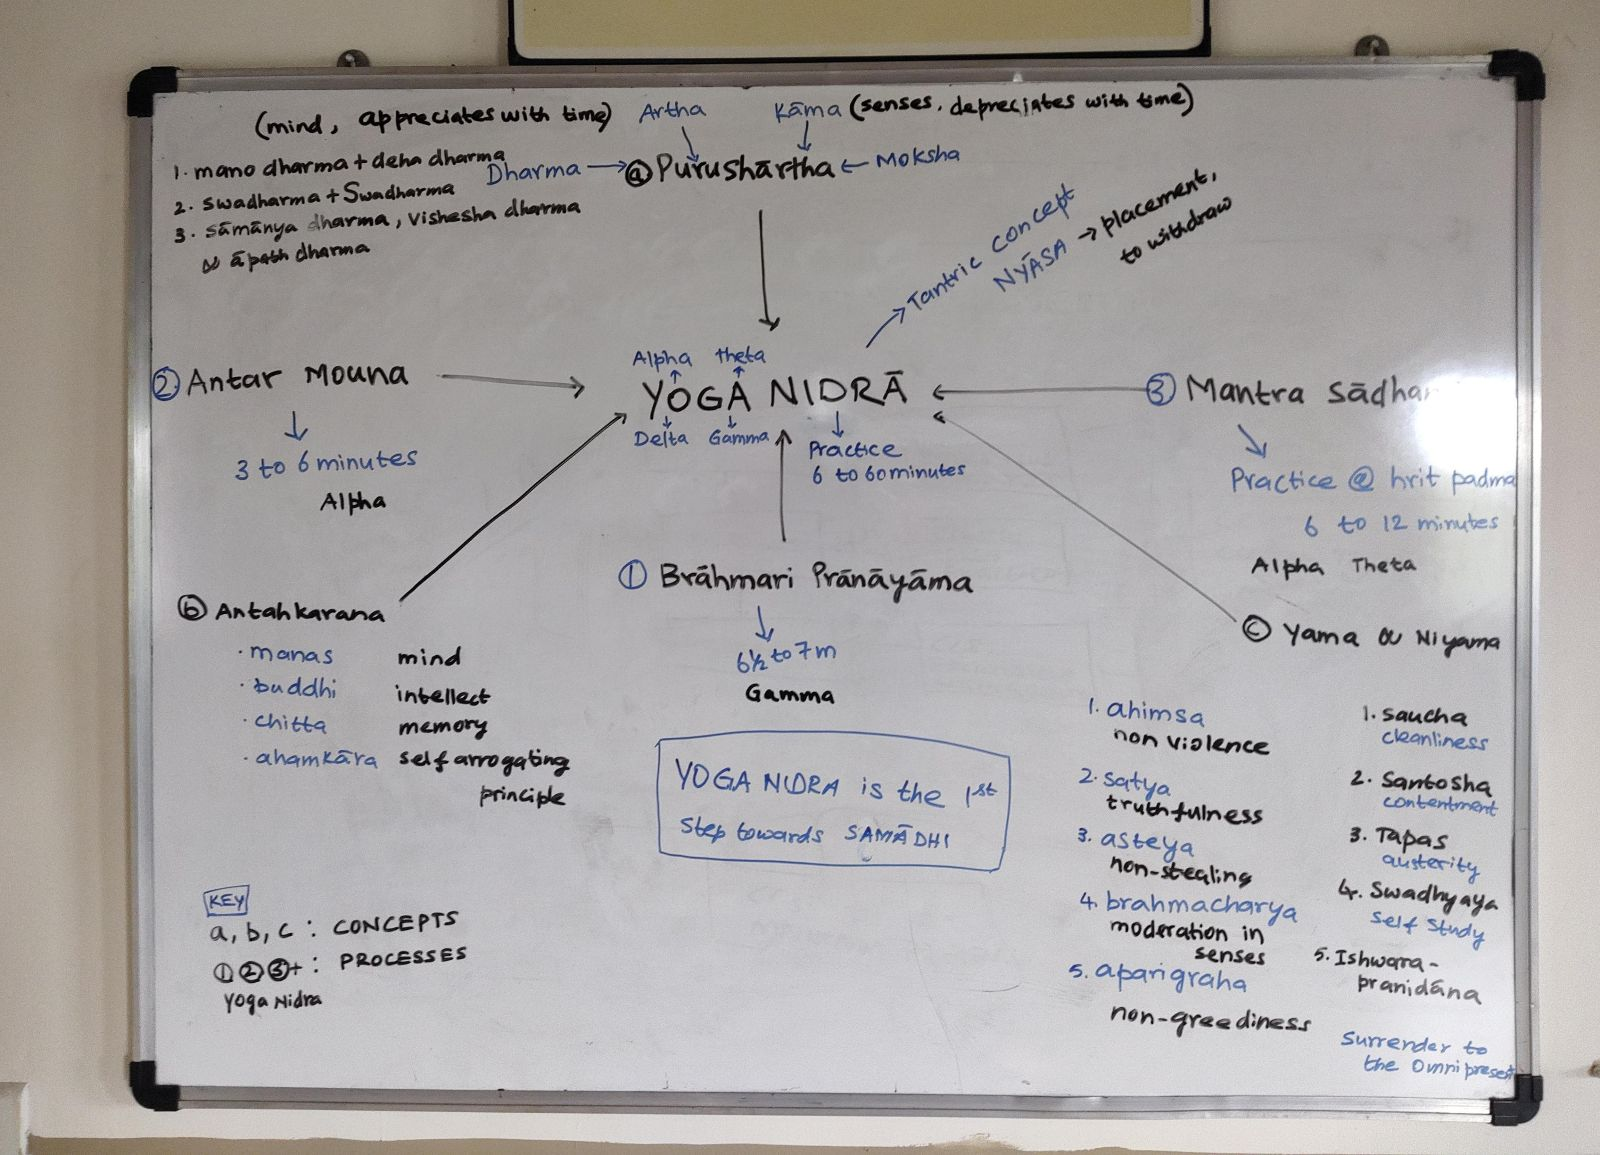
\includegraphics[width=\linewidth,keepaspectratio]{Shrimath_Yoganidra_Mindmap}
	\end{center}	
\end{frame}

%%%%%%%%%%%%%%%%%%%%%%%%%%%%%%%%%%%%%%%%%%%%%%%%%%%%%%%%%%%
\begin{frame}[fragile]\frametitle{Awareness and Waves}
      \begin{itemize}
        \item Awareness is like standing on a seashore.
        \item Waves (thoughts, sounds) come on their own.
        \item No effort is needed to chase them.
        \item In youth, we rush towards experiences.
        \item Maturity: Stand still, waves reach you naturally.
        \item Awareness happens on its own—just be present.
      \end{itemize}
\end{frame}

%%%%%%%%%%%%%%%%%%%%%%%%%%%%%%%%%%%%%%%%%%%%%%%%%%%%%%%%%%%
\begin{frame}[fragile]\frametitle{Yoga Nidra and Nyasa (न्यास)}
      \begin{itemize}
        \item Yoga Nidra originates from \textbf{Nyasa (न्यास)}.
        \item \textbf{Nyasa} (Tantra) = Tried and tested method.
        \item Two meanings: Placement and Withdrawal.
        \item \textbf{Sannyasa (संन्यास)} = Samyak + Nyasa (Perfect withdrawal).
        \item Withdrawing from personal identity; world is family.
        \item Awareness of instructions, no distractions.
      \end{itemize}
\end{frame}

%%%%%%%%%%%%%%%%%%%%%%%%%%%%%%%%%%%%%%%%%%%%%%%%%%%%%%%%%%%
\begin{frame}[fragile]\frametitle{Yoga Nidra and Brain Waves}
      \begin{itemize}
        \item Yoga Nidra balances Alpha and Theta waves.
        \item State: Neither fully asleep nor awake.
        \item Detached witness to distractions.
        \item Enables relaxation, healing, and stress reduction.
        \item Reduces blood pressure and anxiety.
      \end{itemize}
\end{frame}

%%%%%%%%%%%%%%%%%%%%%%%%%%%%%%%%%%%%%%%%%%%%%%%%%%%%%%%%%%%
\begin{frame}[fragile]\frametitle{Mantra (मन्त्र) - The Anchor}
      \begin{itemize}
        \item \textbf{Mantra (मन्त्र)} = Mananat Trayate Iti (मननात् त्रायते इति).
        \item Acts as an anchor in changing life circumstances.
        \item Mood, age, problems change—mantra remains constant.
        \item Regular practice enhances self-healing and mindfulness.
      \end{itemize}
\end{frame}

%%%%%%%%%%%%%%%%%%%%%%%%%%%%%%%%%%%%%%%%%%%%%%%%%%%%%%%%%%%
\begin{frame}[fragile]\frametitle{Dharma (धर्म) - Support and Stability}
      \begin{itemize}
        \item \textbf{Dharma (धर्म)} = That which sustains and supports.
        \item Balance between goal pursuit and emotional resilience.
        \item \textbf{Mano Dharma (मनो धर्म)} = Duty towards the mind.
        \item \textbf{Deha Dharma (देह धर्म)} = Duty towards the body.
        \item Ask: Is my goal aligned with \textbf{Swadharma (स्वधर्म)}?
      \end{itemize}
\end{frame}

%%%%%%%%%%%%%%%%%%%%%%%%%%%%%%%%%%%%%%%%%%%%%%%%%%%%%%%%%%%
\begin{frame}[fragile]\frametitle{Swadharma (स्वधर्म) and Passion}
      \begin{itemize}
        \item Swadharma (self-duty) aligns passion and profession.
        \item If aligned, less marketing needed—service attracts people.
        \item Misalignment = More strategy, planning, and effort.
        \item Example: A hockey player playing cricket for money.
      \end{itemize}
\end{frame}

%%%%%%%%%%%%%%%%%%%%%%%%%%%%%%%%%%%%%%%%%%%%%%%%%%%%%%%%%%%
\begin{frame}[fragile]\frametitle{Yama (यम) and Niyama (नियम)}
      \begin{itemize}
        \item Foundations of Yoga: Yama (यम) and Niyama (नियम).
        \item Useful for refining resolves and desires.
        \item Guides personal discipline and ethical conduct.
      \end{itemize}
\end{frame}

%%%%%%%%%%%%%%%%%%%%%%%%%%%%%%%%%%%%%%%%%%%%%%%%%%%%%%%%%%%
\begin{frame}[fragile]\frametitle{Sankalpa (संकल्प) vs Affirmation}
      \begin{itemize}
        \item Affirmations: Passive, mind-centered, unreliable.
        \item Sankalpa (संकल्प): Active, action-based self-discovery.
        \item Self-chosen—not decided by others.
        \item Rooted in present reality, not abstract desires.
      \end{itemize}
\end{frame}

%%%%%%%%%%%%%%%%%%%%%%%%%%%%%%%%%%%%%%%%%%%%%%%%%%%%%%%%%%%
\begin{frame}[fragile]\frametitle{Framing a Sankalpa (संकल्प)}
      \begin{itemize}
        \item Must be a \textbf{Need}, not just a Want.
        \item Avoid over-ambitious or abstract resolutions.
        \item Focus on what disturbs the mind most.
        \item Resolve must be personal—not for others.
        \item Specific, measurable, and positively framed.
        \item Example: “I need optimum sound sleep.”
      \end{itemize}
\end{frame}

%%%%%%%%%%%%%%%%%%%%%%%%%%%%%%%%%%%%%%%%%%%%%%%%%%%%%%%%%%%
\begin{frame}[fragile]\frametitle{Yoga Nidra - Practical Tips}
      \begin{itemize}
        \item Avoid stiffness—Corpse pose, but not a corpse.
        \item Be still but respond to discomfort (e.g., mosquito).
        \item Use a light blanket—Body temperature may drop.
      \end{itemize}
\end{frame}

%%%%%%%%%%%%%%%%%%%%%%%%%%%%%%%%%%%%%%%%%%%%%%%%%%%%%%%%%%%
\begin{frame}[fragile]\frametitle{Process of Yoga Nidra}
      \begin{itemize}
        \item \textbf{Bhramari (भ्रामरी)} - 7 minutes
        \item \textbf{Antar Mouna (अंतर मौन)} - 2-3 minutes
        \item \textbf{Yoga Nidra (योगनिद्रा)} - 25-35 minutes
        \item \textbf{Mantra Sadhana (मन्त्र साधना)} - 5 minutes
      \end{itemize}
\end{frame}

%%%%%%%%%%%%%%%%%%%%%%%%%%%%%%%%%%%%%%%%%%%%%%%%%%%%%%%%%%%
\begin{frame}[fragile]\frametitle{Levels of Yoga Nidra}
      \begin{itemize}
        \item Level 1: Awareness rotation at joints. (annamaya kosha अन्नमय कोष )
        \item Level 2: Awareness rotation between joints. (annamaya kosha अन्नमय कोष )
        \item Level 3: Awareness rotation + Breath-work. (pranamaya kosha प्राणमय कोष )
        \item Level 4: Awareness rotation + Breath-work + Resolve + Visualizations. (manomaya kosha मनोमय कोष )
      \end{itemize}
\end{frame}


% % %%%%%%%%%%%%%%%%%%%%%%%%%%%%%%%%%%%%%%%%%%%%%%%%%%%%%%%%%%%%%%%%%%%%%%%%%%%%%%%%%%
% \begin{frame}[fragile]\frametitle{}
% \begin{center}
% {\Large References}
% \end{center}
% \end{frame}


%%%%%%%%%%%%%%%%%%%%%%%%%%%%%%%%%%%%%%%%%%%%%%%%%%%%%%%%%%%
\begin{frame}[fragile]\frametitle{References}

Many publicly available sources have been used in the preparation of this content. Some of the salient ones are listed below:

	\begin{itemize}
	\item Master Class on Antar Mouna Level 1 https://www.youtube.com/watch?v=5E0Sw-sAv48
	\item Tapping Grace through Yoga Nidra  https://www.youtube.com/watch?v=4UpYtET2Xes
	\item Building Immunity 2.0 
	\end{itemize}

\end{frame}


% %%%%%%%%%%%%%%%%%%%%%%%%%%%%%%%%%%%%%%%%%%%%%%%%%%%%%%%%%%%
% \begin{frame}[fragile]\frametitle{}

% \begin{center}
% \includegraphics[width=0.8\linewidth,keepaspectratio]{my_yog_back}

% Thanks धन्यवाद
% \end{center}

% \end{frame}

\end{multicols}

\rule{\linewidth}{0.25pt}
\scriptsize
Copyleft \textcopyleft\  Send suggestions to 
\href{http://www.yogeshkulkarni.com}{yogeshkulkarni@yahoo.com}

\end{document}
